\documentclass[11pt,a4paper]{article}

\usepackage[utf8]{inputenc}
\usepackage[T1]{fontenc}
\usepackage[spanish,es-tabla,es-nodecimaldot,es-noshorthands]{babel}
\usepackage{lmodern}
\usepackage{microtype}
\usepackage[margin=2.4cm]{geometry}
\usepackage{amsmath,amssymb,mathtools}
\usepackage{graphicx}
\usepackage{booktabs}
\usepackage{tabularx}
\usepackage{array}
\usepackage{caption}
\usepackage{subcaption}
\usepackage{xcolor}
\usepackage{listings}
\usepackage{enumitem}
\usepackage{tikz}
\usetikzlibrary{arrows.meta,positioning,fit,backgrounds}
\usepackage{cite}
\usepackage[hidelinks]{hyperref}

\graphicspath{{figures/}}
\setlength{\emergencystretch}{3em}
\setlength{\parskip}{0.45em}
\setlength{\parindent}{0pt}
\setlist{itemsep=0.2em,topsep=0.3em}
\captionsetup{font=small,labelfont=bf}

\definecolor{codebg}{HTML}{F4F4F2}
\lstdefinestyle{shell}{
  basicstyle=\ttfamily\small,
  backgroundcolor=\color{codebg},
  frame=single,
  framerule=0pt,
  xleftmargin=0.6em,
  xrightmargin=0.6em,
  breaklines=true,
  columns=fullflexible,
  keepspaces=true,
  showstringspaces=false
}
\lstset{style=shell}

\newcommand{\archivo}[1]{\nolinkurl{#1}}
\makeatletter
\g@addto@macro\UrlBreaks{\do\_}
\makeatother

\title{\textbf{Fresh: probador virtual de barbería con computación gráfica}\\[0.4em]
\large Proyecto final de Computación Gráfica (CS4016)}
\author{Kalos Lazo Mera \qquad Sofía Herrera \qquad Gianpier Segovia\\[0.5em]
\small Universidad de Ingeniería y Tecnología (UTEC)}
\date{Noviembre de 2026}

\begin{document}

\maketitle

\begin{abstract}
\noindent
\textbf{Fresh} (repositorio \emph{BarberStudio}) es una aplicación web que permite probarse barbas, tintes y cortes de pelo sobre una foto propia o con la cámara, antes de ir a la barbería. A partir de los 478 puntos faciales que entrega un modelo preentrenado, el sistema construye una malla de triángulos con una triangulación de Delaunay implementada desde cero (algoritmo de Fortune), deforma texturas de barba real por triángulo con interpolación bilineal propia, recolorea el pelo en el espacio CIELAB, quita y vuelve a crear el pelo para ocho cortes con un relleno \emph{pull-push} y un modelo de cráneo ajustado a cada cabeza, y representa caras, barbas y pelucas como miles de gaussianas en 2D y en 3D, con un visor de \emph{Gaussian Splatting} escrito en WebGL2. El proyecto incluye simulación física de la barba con integración de Verlet, un juego de afeitado, una clasificación de la forma de la cara que sugiere estilos, la segmentación del pelo con un YOLOv8 ajustado por el equipo (mAP50 de máscara de 0{,}968) y una ficha con indicaciones para el barbero. Se valida con 53 pruebas automáticas, integración continua y un contenedor Docker que reproduce la aplicación con un solo comando.

\medskip
\noindent\textbf{Palabras clave:} triangulación de Delaunay, warp afín por partes, espacio de color CIELAB, composición alfa, \emph{pull-push}, \emph{Gaussian Splatting}, integración de Verlet, segmentación de pelo.
\end{abstract}


\tableofcontents
\clearpage

\section{Introducción}

\subsection{Problema}

Cambiar de corte, dejarse la barba o teñirse el pelo son decisiones que se toman a ciegas: el resultado solo se ve cuando ya está hecho y, en el caso de un corte o un tinte, no se puede deshacer. Las aplicaciones que existen para probarse estilos suelen pegar una imagen recortada encima de la foto, sin seguir la forma de la cara ni la luz, o dependen de modelos generativos que inventan la cara completa y requieren servidores con GPU.

Este proyecto aborda el problema con técnicas de computación gráfica: en lugar de generar una imagen nueva, se modela la geometría de la cara y del pelo de la persona y se componen sobre la foto original las capas necesarias (barba, color, pelo corto, piel), de forma que el resultado conserve la identidad, la iluminación y la textura de la foto.

\subsection{Objetivos}

\textbf{Objetivo general.} Construir un producto completo, en forma de aplicación web, que permita probar barbas, tintes y cortes de pelo sobre una foto o con la cámara, usando como núcleo algoritmos de computación gráfica implementados por el equipo.

\textbf{Objetivos específicos.}
\begin{enumerate}
  \item Ajustar plantillas de barba real a cualquier cara mediante una malla de Delaunay propia y un \emph{warp} afín por triángulo.
  \item Recolorear el pelo de forma creíble, respetando su textura y su iluminación.
  \item Simular cortes de pelo cortos (degradados, \emph{taper}, \emph{undercut}, raya marcada, \emph{crew cut} y rapado) quitando el pelo original y reconstruyendo el fondo y la piel.
  \item Representar la cara y el pelo con gaussianas en 2D y en 3D, y renderizarlas en el navegador.
  \item Añadir interacción en tiempo real: modo en vivo con la cámara, física de la barba y un juego de afeitado.
  \item Entregar el sistema con pruebas, integración continua, documentación y un contenedor reproducible.
\end{enumerate}

\subsection{Contribuciones}

Las piezas de visión que detectan la cara y sus puntos (MediaPipe) y la segmentación base del pelo se toman de modelos preentrenados; todo lo demás es implementación propia. En particular:
\begin{itemize}
  \item triangulación de Delaunay con el algoritmo de barrido de Fortune, \emph{warp} afín por triángulo, prueba de interior con coordenadas baricéntricas e interpolación bilineal (sección~\ref{sec:barba});
  \item tinte en CIELAB que separa la luminosidad base del detalle de cada mechón (sección~\ref{sec:tinte});
  \item motor de cortes con relleno \emph{pull-push}, modelo de cráneo, línea del pelo a partir de la frente y sombreado de Lambert (sección~\ref{sec:corte});
  \item detección de barba real por textura y tensor de estructura, y clasificación de la forma de la cara (secciones~\ref{sec:barbatinte} y~\ref{sec:forma});
  \item gaussianas 2D ajustadas con gradientes analíticos y Adam escrito a mano, \emph{Gaussian Splatting} 3D con proyección EWA en WebGL2, exportación a \texttt{.ply} y peluca 3D multivista (secciones~\ref{sec:gauss2d} a~\ref{sec:peluca});
  \item física de la barba con Verlet y restricciones de distancia, y el juego de afeitado con detección de corte por cápsula (secciones~\ref{sec:fisica} y~\ref{sec:juego});
  \item ajuste fino de YOLOv8 para segmentar pelo con Figaro1k y CelebAMask-HQ (sección~\ref{sec:segmentacion}).
\end{itemize}

\begin{figure}[ht]
  \centering
  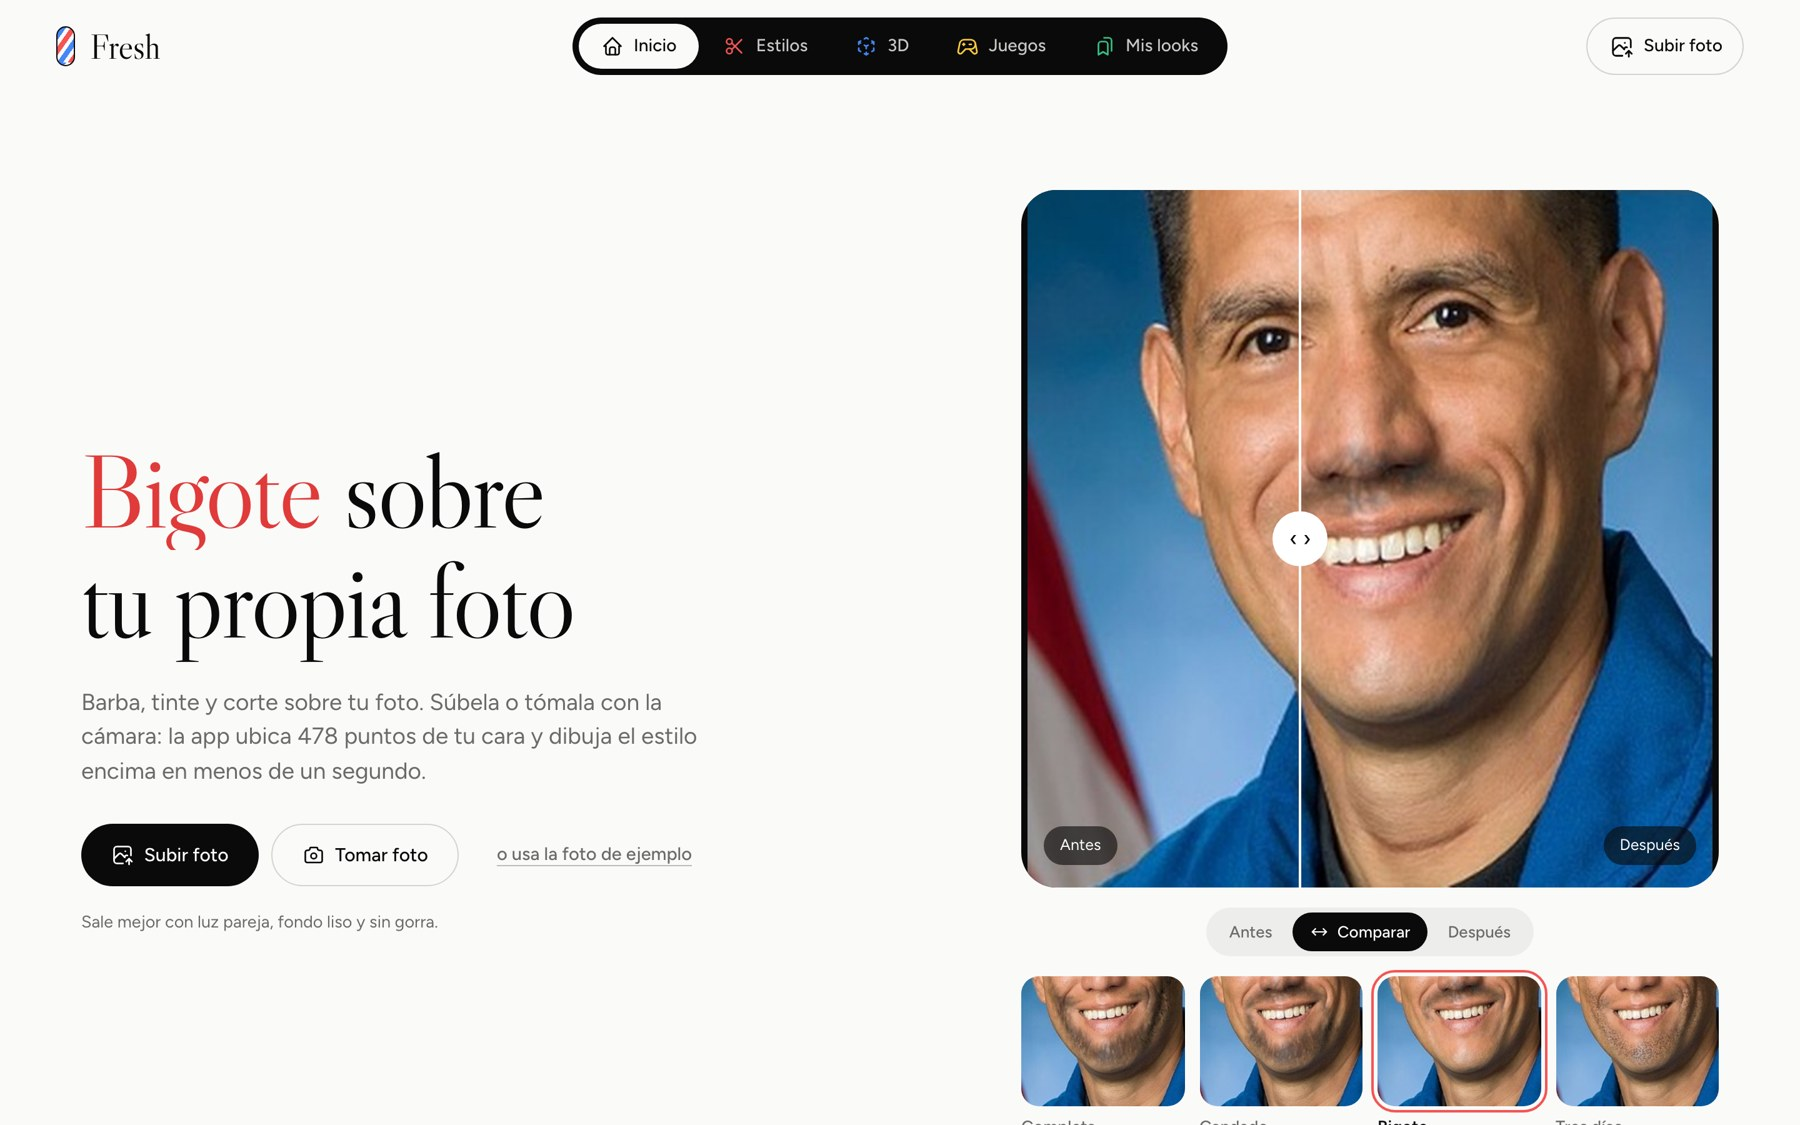
\includegraphics[width=0.92\linewidth]{ui_inicio.jpg}
  \caption{Pantalla de inicio de Fresh. La demostración de la derecha muestra un estilo de barba aplicado sobre un retrato de dominio público de la NASA.}
  \label{fig:inicio}
\end{figure}

\subsection{Relación con los temas del curso}
\label{sec:temas}

Los modelos preentrenados resuelven una sola pregunta: dónde están la cara, el pelo y la mano. Todo lo que la persona ve en pantalla lo calcula código del equipo. En el núcleo del servidor y el visor 3D hay unas 4\,000 líneas de algoritmos gráficos propios y unas 600 líneas que llaman a modelos, es decir, cerca del 87~\% es computación gráfica propia. La tabla~\ref{tab:temas} relaciona cada tema del sílabo del curso con la parte del proyecto que lo aplica.

\begin{table}[ht]
\centering
\small
\begin{tabularx}{\linewidth}{@{}>{\raggedright\arraybackslash}p{3.9cm} X l@{}}
\toprule
Tema del sílabo & Dónde se aplica en Fresh & Sección \\
\midrule
6.1.1 Teoría del color & Tinte en CIELAB; color de la barba en YCrCb; croma que baja en las sombras & \ref{sec:tinte}, \ref{sec:barba} \\
6.1.2 Representación de imágenes & Una foto como suma de gaussianas 2D; capas con alfa & \ref{sec:gauss2d} \\
6.1.3 Muestreo & Pirámide \emph{pull-push}; resolución de trabajo fija; gaussianas por área 3D con muestreo estratificado & \ref{sec:corte}, \ref{sec:espejo} \\
6.1.4 Interpolación & Bilineal propia en el \emph{warp}; baricéntricas para anclar hebras y gaussianas; curvas de Bézier y Chaikin & \ref{sec:barba}, \ref{sec:fisica} \\
6.2.1 Producto vectorial, áreas, Montecarlo & Orientación y área de triángulos; distancia punto--segmento del juego; inicialización aleatoria por importancia de las gaussianas 2D & \ref{sec:juego}, \ref{sec:gauss2d} \\
6.2.2 Línea de barrido y casco convexo & Fortune es un algoritmo de barrido; casco convexo para recortar regiones & \ref{sec:barba} \\
6.2.5 Voronoi y Delaunay & Cada evento de círculo de Fortune es un vértice de Voronoi y un triángulo de Delaunay & \ref{sec:barba} \\
6.3.1 GPU & \emph{Vertex} y \emph{fragment shaders} propios en WebGL2 & \ref{sec:espejo} \\
6.3.2 Procesamiento de mallas & Malla de 478 puntos elevada a 3D; normales y marcos tangentes; parametrización por triángulo con un marco local ortonormal & \ref{sec:espejo}, \ref{sec:lab} \\
6.3.3.1 Rasterización & El \emph{warp} recorre el rectángulo envolvente y prueba cada píxel con baricéntricas & \ref{sec:barba} \\
6.3.3.2 Iluminación y texturas & Lambert en el pelo corto; textura de barba por triángulo; textura de la peluca desde varias vistas & \ref{sec:corte}, \ref{sec:peluca} \\
6.3.3.3 Superficies visibles & Algoritmo del pintor: gaussianas ordenadas de atrás hacia adelante con \emph{counting sort} & \ref{sec:espejo} \\
6.3.3.5 \emph{Gaussian Splatting} & \emph{Render} 3DGS con proyección EWA y exportación \texttt{.ply}; gaussianas 2D ajustadas con gradientes analíticos & \ref{sec:espejo}, \ref{sec:gauss2d} \\
6.4.2 Bordes & Gradientes y tensor de estructura para la barba y la dirección del pelo & \ref{sec:barbatinte}, \ref{sec:peluca} \\
6.4.4 OpenCV & Lectura de imágenes, filtros, detector de Haar & \ref{sec:deteccion} \\
6.4.5--6.4.6 YOLO y ajuste fino & Segmentador de pelo entrenado por el equipo & \ref{sec:segmentacion} \\
\bottomrule
\end{tabularx}
\caption{Temas del sílabo de CS4016 que aplica el proyecto.}
\label{tab:temas}
\end{table}

Quedan fuera la transformada de Fourier (6.1.5), los \emph{kd-trees} (6.2.4), el \emph{windowing} (6.2.6), CUDA (6.3.1.2) y el trazado de rayos (6.3.3.3--6.3.3.4).

\subsection{Organización del documento}

La sección~\ref{sec:fundamentos} resume los fundamentos teóricos. La sección~\ref{sec:metodologia} describe los requisitos y la metodología de trabajo, y la sección~\ref{sec:arquitectura}, la arquitectura del sistema. La sección~\ref{sec:implementacion} detalla cada módulo con sus algoritmos, decisiones y limitaciones. La sección~\ref{sec:herramientas} indica qué herramienta resolvió cada parte, y la sección~\ref{sec:reproduccion} explica paso a paso cómo reproducir el proyecto. Los resultados se presentan en la sección~\ref{sec:resultados}, las limitaciones en la sección~\ref{sec:limitaciones} y las conclusiones en la sección~\ref{sec:conclusiones}.

\section{Fundamentos}
\label{sec:fundamentos}

Esta sección resume la teoría que usa el proyecto, con la notación que se emplea en el resto del documento.

\subsection{Imágenes, espacios de color y composición}

Una imagen digital es una función muestreada $I:\{0,\dots,W-1\}\times\{0,\dots,H-1\}\to[0,255]^3$ \cite{gonzalez2018}. Además de RGB, el proyecto usa dos espacios de color:
\begin{itemize}
  \item \textbf{YCrCb}, que separa la luminancia $Y$ de dos componentes de croma $C_r$ y $C_b$. Permite cambiar el tono de una barba sin alterar su brillo.
  \item \textbf{CIELAB}, diseñado para que distancias iguales correspondan aproximadamente a diferencias de color percibidas iguales \cite{cie2004,fairchild2013}. $L^*$ es la luminosidad, y $a^*$ y $b^*$ son los ejes verde--rojo y azul--amarillo. Cambiar $a^*,b^*$ manteniendo la variación de $L^*$ recolorea sin perder la textura.
\end{itemize}

La composición de una capa de color $c$ con opacidad $\alpha\in[0,1]$ sobre un fondo $b$ sigue el operador \emph{over} de Porter y Duff \cite{porter1984}:
\begin{equation}
  C = \alpha\,c + (1-\alpha)\,b.
\end{equation}
Para la barba también se usa el modo \emph{multiply}, $C=(1-\alpha)\,b+\alpha\,b\,m$ con $m\in[0,1]$, que oscurece la piel sin tapar sus luces y sombras.

\subsection{Muestreo, interpolación y coordenadas baricéntricas}

Cuando una transformación geométrica lleva un píxel de salida a una posición no entera $(x,y)$ de la imagen de origen, el valor se reconstruye con interpolación bilineal \cite{marschner2016}. Con $x_0=\lfloor x\rfloor$, $y_0=\lfloor y\rfloor$, $w_x=x-x_0$ y $w_y=y-y_0$:
\begin{equation}
  v=(1-w_x)(1-w_y)P_{00}+w_x(1-w_y)P_{10}+(1-w_x)w_yP_{01}+w_xw_yP_{11}.
\end{equation}

Un punto $p$ dentro de un triángulo $ABC$ se escribe como $p=\lambda_1A+\lambda_2B+\lambda_3C$, con $\lambda_1+\lambda_2+\lambda_3=1$. Estas son sus coordenadas baricéntricas: el punto está dentro del triángulo si y solo si $\lambda_i\ge0$ para todo $i$. Además, si los vértices se mueven, $p'=\lambda_1A'+\lambda_2B'+\lambda_3C'$ es el mismo punto ``pegado'' a la superficie. El proyecto usa esta propiedad para anclar pelos y gaussianas a la cara.

\subsection{Triangulación de Delaunay y algoritmo de Fortune}

Dado un conjunto de puntos $P$ en el plano, la triangulación de Delaunay es aquella en la que ningún punto de $P$ cae dentro del círculo circunscrito de ningún triángulo \cite{delaunay1934}. Entre todas las triangulaciones posibles, maximiza el ángulo mínimo \cite{deberg2008}; por eso evita triángulos muy finos, que deformarían mal una textura. Es el grafo dual del diagrama de Voronoi.

El algoritmo de Fortune \cite{fortune1987} construye el diagrama de Voronoi en $O(n\log n)$ con una línea de barrido. Mantiene una \emph{beach line} formada por arcos de parábola, uno por cada sitio ya visitado, y procesa dos tipos de eventos en una cola de prioridad:
\begin{itemize}
  \item \textbf{evento de sitio}: la línea alcanza un punto nuevo y aparece un arco;
  \item \textbf{evento de círculo}: un arco se reduce a ancho cero y desaparece. Su posición es un vértice de Voronoi, y los tres sitios que lo definen tienen un círculo circunscrito vacío, es decir, forman un triángulo de Delaunay.
\end{itemize}
Las alternativas incrementales, como Bowyer--Watson \cite{bowyer1981,watson1981}, insertan los puntos uno por uno y rehacen los triángulos cuyo círculo contiene el punto nuevo.

\subsection{Transformación afín por triángulo}

Una transformación afín $T(x,y)=(a x+b y+c,\; d x+e y+f)$ queda determinada por tres pares de puntos. Por eso, una malla de triángulos en dos posiciones (origen y destino) define un \emph{warp} afín por partes \cite{szeliski2022}: cada triángulo de la textura se lleva a su triángulo correspondiente sobre la cara. Para no dejar huecos, se recorre cada píxel del triángulo de destino y se calcula con la transformación inversa de dónde leer en el origen (\emph{backward mapping}).

\subsection{Gaussianas, \emph{splatting} y proyección EWA}

Una gaussiana anisótropa 3D con centro $\mu$ y covarianza $\Sigma$ tiene densidad $G(x)=\exp\!\left(-\tfrac12(x-\mu)^\top\Sigma^{-1}(x-\mu)\right)$. \emph{3D Gaussian Splatting} \cite{kerbl2023} representa una escena como un conjunto de gaussianas con color y opacidad. Para dibujarlas, cada gaussiana se proyecta a la pantalla con la aproximación EWA \cite{zwicker2001}: si $W$ es la rotación de la vista y $J$ la jacobiana de la proyección en el centro, la covarianza en pantalla es
\begin{equation}
  \Sigma_{2D}=J\,W\,\Sigma\,W^\top J^\top.
\end{equation}
Las gaussianas proyectadas se ordenan de atrás hacia adelante y se componen con
\begin{equation}
  C=\sum_i c_i\,\alpha_i\prod_{j<i}(1-\alpha_j).
\end{equation}
En 2D, GaussianImage \cite{zhang2024} representa una imagen como suma de gaussianas sin orden, ajustadas por descenso de gradiente. El proyecto implementa ambas ideas desde cero, sin bibliotecas de diferenciación automática.

\subsection{Simulación con Verlet y dinámica basada en posiciones}

La integración de Verlet \cite{verlet1967} avanza una partícula usando su posición actual y la anterior: $x_{t+h}=x_t+(x_t-x_{t-h})+a\,h^2$. No guarda la velocidad explícitamente, por lo que imponer restricciones consiste simplemente en mover posiciones. La dinámica basada en posiciones (PBD) \cite{jakobsen2001,muller2007} aprovecha esto: después de integrar, proyecta las partículas para que cumplan restricciones como la distancia fija entre nodos de una cuerda. Es estable incluso con pasos de tiempo grandes, algo necesario a 10 cuadros por segundo.

\subsection{Rellenado de regiones}

Cuando se quita pelo que tapaba el fondo, hay que inventar los píxeles faltantes. El \emph{inpainting} por \emph{fast marching} de Telea \cite{telea2004} propaga los valores del borde hacia adentro. El método \emph{pull-push} \cite{gortler1996} construye una pirámide: en la fase \emph{pull} promedia, en cada nivel, solo los píxeles conocidos ponderados por su peso; en la fase \emph{push} rellena los huecos de cada nivel fino con el nivel grueso. La diferencia clave para este proyecto es que en \emph{pull-push} se elige qué píxeles cuentan como conocidos.

\subsection{Orientación local: el tensor de estructura}

Con los gradientes $g_x,g_y$ de una imagen, el tensor de estructura promedia en una vecindad la matriz $J=\begin{pmatrix}g_x^2 & g_xg_y\\ g_xg_y & g_y^2\end{pmatrix}$ \cite{bigun1987}. Sus autovalores $\lambda_1\ge\lambda_2$ describen la textura local:
\begin{itemize}
  \item la \textbf{orientación dominante} es $\theta=\tfrac12\operatorname{atan2}(2J_{xy},J_{xx}-J_{yy})$;
  \item la \textbf{coherencia} $(\lambda_1-\lambda_2)/(\lambda_1+\lambda_2)$ vale cerca de 1 en un borde recto y largo, y es menor en una textura de trazos en todas direcciones, como la barba.
\end{itemize}

\subsection{Detección y segmentación con modelos}

El detector de Viola--Jones \cite{viola2001} clasifica ventanas con una cascada de rasgos de Haar. MediaPipe \cite{lugaresi2019} ofrece, entre otros, un modelo de malla facial de 468 puntos con profundidad, más 10 puntos de iris \cite{kartynnik2019}, y un segmentador por clases (fondo, pelo, piel del cuerpo, piel de la cara, ropa y accesorios). YOLO \cite{redmon2016} es una familia de detectores de una sola pasada; YOLOv8 \cite{jocher2023} agrega una cabeza de segmentación por instancia. Las máscaras gruesas se ajustan a los bordes reales con el filtro guiado de He \emph{et al.} \cite{he2013}, que usa la propia foto como guía.

\section{Requisitos y metodología}
\label{sec:metodologia}

\subsection{Requisitos}

\textbf{Funcionales.}
\begin{enumerate}[label=RF\arabic*.]
  \item Cargar una foto, tomarla con la cámara o usar una foto de ejemplo, y compartirla entre todas las herramientas.
  \item Aplicar cuatro estilos de barba con densidad ajustable.
  \item Teñir el pelo con siete colores o un color libre y, opcionalmente, también la barba.
  \item Aplicar ocho cortes: degradado bajo, medio y alto, \emph{taper}, \emph{undercut}, raya marcada, \emph{crew cut} y rapado.
  \item Combinar barba, tinte y corte en un mismo resultado.
  \item Comparar antes y después, guardar looks y generar una ficha para el barbero.
  \item Sugerir estilos según la forma de la cara.
  \item Mostrar la cabeza y una peluca en 3D, girables y exportables.
  \item Probar estilos en vivo con la cámara, con física de la barba y un juego de afeitado.
\end{enumerate}

\textbf{No funcionales y restricciones.}
\begin{enumerate}[label=RNF\arabic*.]
  \item Sin GPU: todo el procesamiento corre en CPU.
  \item Respuesta de menos de 2~s por foto en el contenedor, para fotos de celular de hasta 4000~px.
  \item Interfaz sin paso de compilación (HTML, CSS y JavaScript nativos), para que el proyecto sea fácil de reproducir en el curso.
  \item La interfaz se adapta al celular.
  \item Reproducible con un solo comando mediante Docker.
\end{enumerate}

\subsection{Metodología}

El equipo trabajó de forma iterativa e incremental, con entregas funcionales en cada iteración. Cada funcionalidad nueva siguió el mismo ciclo: propuesta escrita en \archivo{docs/}, implementación en \archivo{backend/app/core}, pruebas automáticas, revisión visual sobre retratos de prueba y documentación técnica. Las fechas salen del historial de \texttt{git}:

\begin{table}[ht]
\centering
\small
\begin{tabularx}{\linewidth}{@{}l X@{}}
\toprule
Iteración & Contenido \\
\midrule
1 (30 ago -- 1 sep) & Arquitectura FastAPI + interfaz, detección de cara y puntos, tinte inicial, preparación de datos y entrenamiento de YOLO. \\
2 (16 -- 19 sep) & Barba con plantillas, Delaunay propio y \emph{warp}; primera versión de transferencia de pelo. \\
3 (21 oct -- 6 nov) & Física de la barba, gaussianas 2D, juego, espejo 3D, laboratorio, peluca 3D multivista con color y recorte. \\
4 (9 -- 10 nov) & Producto: interfaz Fresh, Docker e integración continua, cámara, motor de cortes, combinación de looks, forma de cara, tinte de barba y YOLO propio en la aplicación. \\
\bottomrule
\end{tabularx}
\caption{Iteraciones del proyecto.}
\label{tab:iteraciones}
\end{table}

\textbf{Control de versiones y calidad.} El código vive en un repositorio git compartido por los tres integrantes. En las primeras iteraciones cada uno integraba su módulo directamente; desde la iteración 4, los cambios entran a \texttt{main} por \emph{pull requests} con una rama por funcionalidad. GitHub Actions ejecuta las pruebas en cada \emph{push} y en cada \emph{pull request}. Las convenciones de código están escritas en \archivo{AGENTS.md}:
\begin{itemize}
  \item la lógica vive en \archivo{backend/app/core};
  \item los \emph{endpoints} quedan delgados;
  \item los datasets y pesos pesados no se versionan, con dos excepciones: los modelos de MediaPipe y \archivo{hair_best.pt}, de 6{,}5~MB.
\end{itemize}

\textbf{Verificación de requisitos.} Cada requisito se verificó de tres maneras complementarias:
\begin{itemize}
  \item 47 pruebas automáticas (sección~\ref{sec:pruebas});
  \item recorridos completos en el navegador: Chrome sin ventana controlado por el protocolo DevTools, con cámara simulada;
  \item revisión visual de cuadrículas de resultados sobre 26 caras distintas: piel clara, morena y negra; pelo liso, rizado, largo y corto; con flequillo y con entradas.
\end{itemize}
Los tiempos se midieron sobre el contenedor (sección~\ref{sec:resultados}).

\subsection{Organización del equipo}

El equipo se dividió por módulos, con un responsable principal por cada uno. La tabla~\ref{tab:aportes} resume los aportes según el historial del repositorio.

\begin{table}[ht]
\centering
\small
\begin{tabularx}{\linewidth}{@{}l X@{}}
\toprule
Integrante & Aportes principales \\
\midrule
Kalos Lazo Mera & Arquitectura del backend y de la API; tinte; preparación de datos y entrenamiento de YOLO; interfaz Fresh; motor de cortes; combinación de looks; forma de cara; tinte de barba; Docker, integración continua y pruebas. \\
Gianpier Segovia & Barba con plantillas reales; Delaunay de Fortune; \emph{warp} afín; física de la barba; gaussianas 2D; juego de afeitado; espejo 3D; laboratorio (compartido). \\
Sofía Herrera & Peluca 3D: máscara de transferencia, escaneo con la cámara, peluca de gaussianas multivista, cara 3D, cabeza sin pelo y estudio de color y recorte; laboratorio (compartido). \\
\bottomrule
\end{tabularx}
\caption{Aportes por integrante.}
\label{tab:aportes}
\end{table}

\section{Arquitectura del sistema}
\label{sec:arquitectura}

Fresh es una aplicación cliente--servidor. El mismo proceso de Python sirve la interfaz web y la API, de modo que basta con abrir \texttt{http://localhost:8000}. La figura~\ref{fig:arquitectura} muestra las capas.

\begin{figure}[ht]
\centering
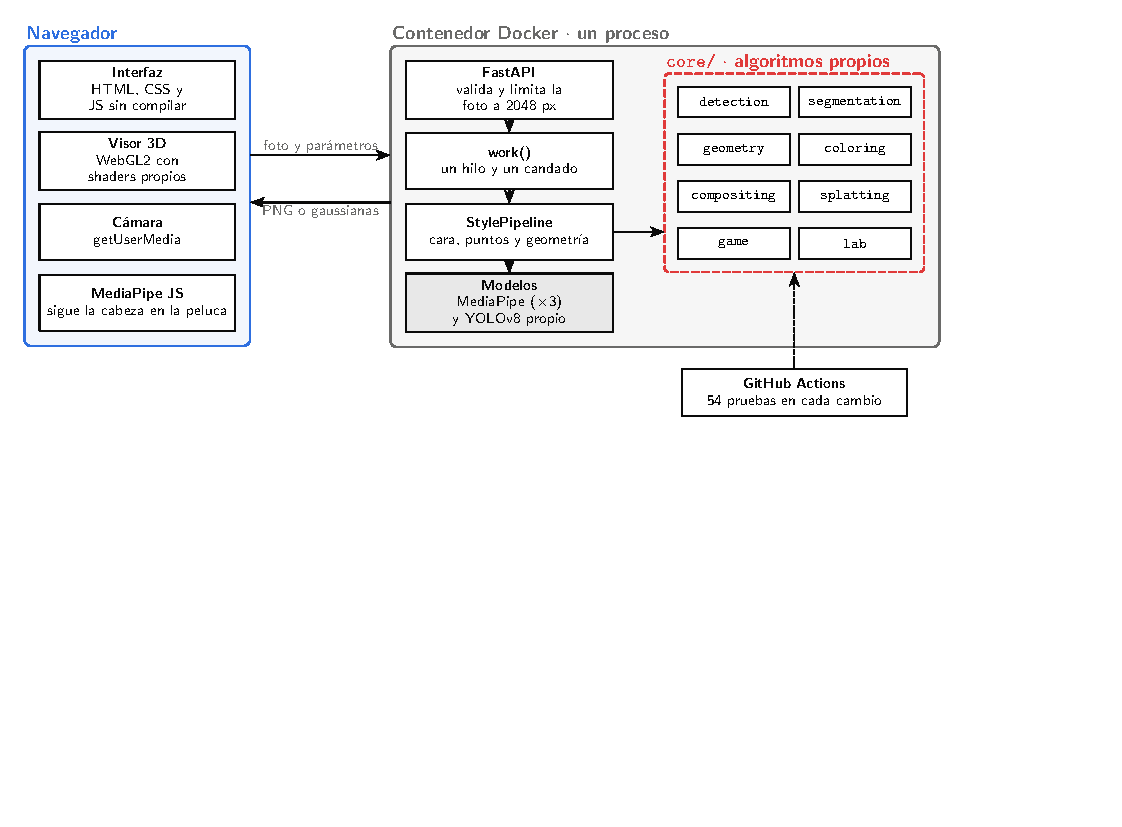
\includegraphics[width=\linewidth]{diagrama_arquitectura.pdf}
\caption{Arquitectura de Fresh. El navegador envía la foto y los parámetros; un único proceso de FastAPI, dentro de un contenedor Docker, pasa cada llamada por \texttt{work()} al pipeline y devuelve la imagen procesada o las gaussianas que dibuja el visor WebGL2.}
\label{fig:arquitectura}
\end{figure}

\subsection{Servidor}

El servidor está escrito en Python con FastAPI \cite{fastapi}, OpenCV \cite{bradski2000} y NumPy \cite{harris2020}. Se organiza en tres niveles:
\begin{itemize}
  \item \textbf{API} (\archivo{api/routes.py}): valida parámetros, decodifica la imagen, la reduce a un lado máximo de 2048~px y devuelve un PNG o datos binarios. No contiene lógica gráfica.
  \item \textbf{Orquestación} (\archivo{core/pipeline.py}): la clase \texttt{StylePipeline} carga los modelos una sola vez y encadena los pasos comunes de cada herramienta: cara, puntos, geometría de la cabeza y probabilidades de segmentación.
  \item \textbf{Módulos} (\archivo{core/*}): cada técnica vive en su propio paquete, sin depender de la API, y es lo que prueban los tests unitarios.
\end{itemize}

\textbf{Un solo proceso, a propósito.} El modo en vivo, la prueba de la peluca y el juego guardan estado entre cuadros: el ancla de la cara, el color del pelo y la ronda en curso. Por eso el servidor corre un único proceso de \texttt{uvicorn}; con dos, cada cuadro caía en uno distinto y el juego alternaba entre dos partidas. Cada llamada al \emph{pipeline} se ejecuta en un hilo aparte detrás de un candado, así el servidor sigue respondiendo mientras procesa una foto y los modelos nunca se usan desde dos hilos a la vez.

\subsection{Interfaz}

La interfaz no usa \emph{frameworks} ni compilación:
\begin{itemize}
  \item \archivo{index.html} define los paneles;
  \item \archivo{app.js} llama a la API de cada herramienta;
  \item \archivo{ui.js} implementa la navegación, la foto compartida, la combinación de looks, la ficha y las sugerencias;
  \item \archivo{splat3d.js} es el visor de gaussianas en WebGL2 \cite{khronos2017}.
\end{itemize}
Los datos personales (looks guardados) se quedan en el \texttt{localStorage} del navegador.

\subsection{Flujo de una petición}

Por ejemplo, al aplicar un degradado medio:
\begin{enumerate}
  \item el navegador envía \texttt{POST /api/haircut} con la foto, \texttt{style=mid-fade} y la intensidad;
  \item el servidor detecta la cara, calcula los 478 puntos y los convierte al formato de 68 puntos, construye la geometría de la cabeza y segmenta el pelo;
  \item el módulo \archivo{compositing/haircut.py} renderiza el corte sobre un recorte de la cabeza a una resolución de trabajo fija y lo devuelve a la resolución original;
  \item la interfaz muestra el resultado en el comparador antes/después.
\end{enumerate}
La lista completa de \emph{endpoints} está en el anexo~\ref{sec:anexo-api}.

\section{Implementación}
\label{sec:implementacion}

Esta sección describe cada módulo:
\begin{itemize}
  \item qué resuelve y cómo funciona;
  \item las decisiones que se tomaron y por qué;
  \item las limitaciones conocidas.
\end{itemize}
Las rutas de archivos son relativas a \archivo{backend/app/core/} salvo que se indique otra cosa.

\subsection{Detección de la cara y de los puntos faciales}
\label{sec:deteccion}

\textbf{Cara.} En el modo foto, la cara se ubica con el clasificador de Haar de OpenCV \cite{viola2001} (\archivo{detection/face_detector.py}) y se elige la de mayor área. En el modo en vivo no se usa, porque falló en el 30~\% de 2695 cuadros al girar la cabeza; ahí la cara sale directamente de los puntos.

\textbf{Puntos.} El modelo \emph{Face Landmarker} de MediaPipe \cite{kartynnik2019} devuelve 478 puntos normalizados con profundidad. Este modelo no lo entrenamos: se usa solo para inferencia. Como el resto del sistema se diseñó sobre el estándar iBUG de 68 puntos, \archivo{detection/landmarks.py} los convierte así:
\begin{itemize}
  \item \textbf{mandíbula}: los 23 puntos del contorno inferior se remuestrean por longitud de arco a 17 puntos equiespaciados (longitud acumulada e interpolación lineal);
  \item \textbf{cejas, ojos, nariz y boca}: 51 puntos salen de una tabla de correspondencias.
\end{itemize}
La malla completa con profundidad se conserva para el espejo 3D, el laboratorio y la forma de la cara.

\textbf{Estabilidad en vivo.} En video se usa el modo de seguimiento de MediaPipe y un filtro One-Euro \cite{casiez2012}. Es un pasa-bajos cuyo corte crece con la velocidad:
\begin{equation}
  f_c=f_{\min}+\beta\,|\hat{\dot x}|,\qquad \alpha=\frac{1}{1+\tau/\Delta t},\quad \tau=\frac{1}{2\pi f_c}.
\end{equation}
Con la cara quieta suaviza fuerte y elimina el temblor; con la cara en movimiento sube el corte y no se queda atrás.

Si MediaPipe pierde la cara durante un cuadro, se reutilizan los últimos puntos hasta tres cuadros. Se desplazan con la traslación global estimada por correlación de fase sobre la zona de la cara.

\textbf{Geometría de la cabeza.} A partir de los 68 puntos, \archivo{segmentation/transfer_mask.py} calcula:
\begin{itemize}
  \item el centro entre las orejas a la altura de los ojos;
  \item el ancho de la cabeza $w$: la distancia 3D entre orejas, que no se encoge al girar;
  \item el giro en el plano;
  \item la altura de las cejas y del mentón;
  \item el polígono de la cara, formado por la mandíbula y las cejas.
\end{itemize}
Todos los módulos de pelo trabajan en un marco normalizado $(x,y)$ medido en anchos de cabeza, con origen entre las orejas a la altura de los ojos, $y$ hacia abajo y rotado con la cabeza. Así los parámetros valen igual para una foto de 600~px y para una de 4000~px.

\subsection{Segmentación del pelo}
\label{sec:segmentacion}

El proyecto tiene dos segmentadores de pelo intercambiables.

\textbf{MediaPipe multiclase.} El modelo \emph{selfie multiclass} de MediaPipe (\archivo{segmentation/mp_segmenter.py}) da, por píxel, la probabilidad de seis clases: fondo, pelo, piel del cuerpo, piel de la cara, ropa y otros. Se aplica sobre una ventana alrededor de la cabeza a $256\times256$~px y se reescala. A diferencia de un umbral de oscuridad, distingue el pelo de un fondo oscuro. Las probabilidades de fondo y de piel también se usan en el corte (sección~\ref{sec:corte}).

\textbf{YOLOv8 ajustado por el equipo.} Se ajustó un YOLOv8n-seg \cite{jocher2023}, preentrenado en COCO, para segmentar pelo:
\begin{itemize}
  \item \textbf{datos}: 9450 imágenes de Figaro1k \cite{svanera2016} y CelebAMask-HQ \cite{lee2020}, convertidas a polígonos con \archivo{backend/training/prepare_hair_dataset.py};
  \item \textbf{entrenamiento}: en Google Colab con \archivo{barberstudio_colab.ipynb} (unas 3{,}5~h en una GPU T4 gratuita);
  \item \textbf{resultado}: mAP50 de máscara de 0{,}968 en validación;
  \item \textbf{ajuste al borde}: la máscara se ajusta al borde real con un filtro guiado \cite{he2013} (\archivo{segmentation/mask_refiner.py}). Después se descartan los píxeles cuyo color se parece más al anillo de fondo que al interior del pelo.
\end{itemize}

En el panel de tinte, el usuario elige el modelo. Si elige YOLO, el servidor calcula también la máscara de MediaPipe y devuelve la intersección sobre unión (IoU) entre ambas. Sobre retratos de prueba, la coincidencia va de 0{,}58 a 0{,}96 (sección~\ref{sec:resultados}).

\subsection{Forma de la cara y sugerencias}
\label{sec:forma}

\archivo{geometry/face_shape.py} clasifica la cara en ovalada, redonda, cuadrada, alargada o corazón. Usa la malla 3D, así que las medidas no dependen de la distancia a la cámara. Se divide todo por el ancho de los pómulos $C=\lVert p_{234}-p_{454}\rVert$:
\begin{align}
  \text{largo}&=\frac{\lVert p_{10}-p_{152}\rVert}{C}, &
  \text{frente}&=\frac{\lVert p_{54}-p_{284}\rVert}{C}, &
  \text{mandíbula}&=\frac{\lVert p_{172}-p_{397}\rVert}{C},
\end{align}
más el ángulo medio del contorno en las esquinas de la mandíbula (puntos 172 y 397, entre la mejilla y el mentón). La figura~\ref{fig:forma} muestra las medidas sobre una cara.

Las proporciones faciales humanas varían poco \cite{farkas1994}, así que un umbral fijo clasificaría casi todas las caras en la misma forma. Por eso se calibró con 419 caras de CelebAMask-HQ: cada medida se expresa como desviación $z$ respecto de la media de esa muestra. Las reglas, en orden, son:
\begin{itemize}
  \item \textbf{alargada}: $z_{\text{largo}}>1$ y $z_{\text{mand}}<0{,}5$;
  \item \textbf{corazón}: $z_{\text{frente}}>0{,}6$ y $z_{\text{mand}}<-0{,}6$;
  \item \textbf{cuadrada o redonda}: $z_{\text{mand}}>0{,}4$ y $z_{\text{largo}}<0{,}6$; es cuadrada si el ángulo de la mandíbula es cerrado y redonda en caso contrario;
  \item \textbf{redonda} también si $z_{\text{largo}}<-0{,}9$;
  \item \textbf{ovalada} en cualquier otro caso.
\end{itemize}
En la muestra, la forma más frecuente es la ovalada (37~\%). El 73~\% de las caras con el atributo ``rellena'' del dataset quedan como redondas o cuadradas.

Cada forma lleva una recomendación de cortes y barbas, basada en la práctica de barbería: alargar una cara redonda con lados cortos, ensanchar una cara alargada con la barba completa, etc. La interfaz las marca como ``Te queda''. Es una heurística: no es una regla médica ni estética universal.

\begin{figure}[ht]
  \centering
  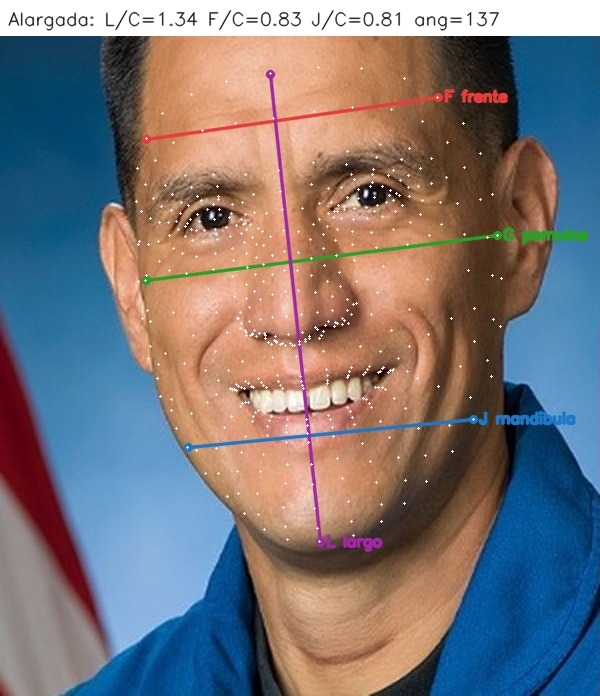
\includegraphics[width=0.42\linewidth]{forma_cara.jpg}
  \caption{Medidas sobre la malla 3D: frente (F), pómulos (C), mandíbula (J) y largo (L). Arriba, las proporciones y la forma resultante.}
  \label{fig:forma}
\end{figure}

\subsection{Barba con plantillas reales}
\label{sec:barba}

La barba no se dibuja desde cero: se ajusta una plantilla real a la cara de la persona.

\textbf{Plantillas.} \archivo{backend/training/harvest_beards.py} recorre CelebAMask-HQ una sola vez y procesa cada foto así:
\begin{enumerate}
  \item filtra por atributos: hombre, sin sombrero, nítida, y clasifica en barba completa, candado, bigote o tres días;
  \item detecta los 68 puntos de la cara;
  \item calcula por píxel un alfa de pelo, ``más oscuro que su entorno'': $\alpha=\operatorname{clip}\big((Y_{\text{local}}-10-Y)/14,0,1\big)$;
  \item descarta las plantillas asimétricas o con poco contraste;
  \item guarda el recorte BGRA, sus puntos y el tono de piel en YCrCb.
\end{enumerate}
Quedan 10 plantillas. En tiempo de ejecución se elige, dentro del estilo pedido, la de croma de piel más cercano al del usuario.

\textbf{Malla.} A los 68 puntos se suman 15 puntos virtuales bajo la mandíbula, para que la barba bajo el mentón quede dentro de la malla. Sobre los 83 puntos se calcula la triangulación de Delaunay con nuestra implementación del algoritmo de Fortune (\archivo{geometry/delaunay_fortune.py}):
\begin{itemize}
  \item una cola de prioridad (\texttt{heapq}) guarda los eventos de sitio y de círculo;
  \item cada evento de círculo aporta directamente un triángulo, sin construir el diagrama de Voronoi completo.
\end{itemize}
También hay una implementación de Bowyer--Watson (\archivo{geometry/delaunay.py}) que da el mismo resultado; se usó para validar.

\textbf{\emph{Warp} afín por triángulo.} \archivo{geometry/warp.py} reemplaza a las funciones de OpenCV por una versión propia. Para cada triángulo:
\begin{enumerate}
  \item resuelve el sistema $3\times3$ de la afín inversa (destino a origen);
  \item recorre los píxeles del rectángulo envolvente del triángulo de destino y se queda con los que tienen coordenadas baricéntricas no negativas;
  \item lee el origen con interpolación bilineal.
\end{enumerate}
Solo se procesan los triángulos cercanos a la barba.

\textbf{Color.} El color del pelo se mide como la mediana dentro de la máscara de pelo y se pasa a YCrCb. A la nube de color de la barba deformada se le suma un desplazamiento constante hacia ese color. Un desplazamiento, y no un reemplazo, conserva la variación interna, es decir, los pelos. El croma se limita a tonos naturales para que un fondo azul no tiña la barba.

\textbf{Región y borde.} La región de cada estilo se arma con polígonos y elipses sobre los 68 puntos:
\begin{itemize}
  \item el bigote es una banda en arco que sigue una curva de Bézier cuadrática;
  \item a la región se le restan los labios y se recorta al casco convexo de la cara;
  \item el borde se suaviza con un \emph{feather} orgánico: distancia al borde (\emph{distance transform}) más ruido.
\end{itemize}

\textbf{Composición en tres capas.} Sea $\rho$ la densidad elegida y $\alpha_r$ el alfa de la región:
\begin{enumerate}
  \item \textbf{cuerpo}: \emph{multiply} con $m=0{,}35+0{,}65\,c/255$ y ruido anisótropo orientado según la dirección del pelo. La luz de la piel sigue viéndose a través de la barba;
  \item \textbf{hebras}: curvas de Bézier cuadráticas que siguen un campo de dirección hacia abajo y hacia afuera. Su cantidad es proporcional a $\rho$, hasta 9000;
  \item \textbf{detalle}: se transfiere solo la alta frecuencia de la plantilla, $\text{plantilla}-G_\sigma(\text{plantilla})$. Así se conservan los pelos reales sin traer el brillo ni el color de la otra persona. Se descartó un \emph{Poisson blending} \cite{perez2003} porque igualaba el brillo con el borde y aclaraba la barba.
\end{enumerate}
El estilo ``tres días'' reemplaza las capas 2 y 3 por un grano de 1~px cuyo umbral baja al subir la densidad. La figura~\ref{fig:barba} muestra los cuatro estilos.

\textbf{En vivo.} La textura se genera una vez y se ancla a la malla de referencia (\texttt{LiveAnchor}):
\begin{itemize}
  \item en cada cuadro, los ruidos se deforman con el mismo \emph{warp};
  \item cada hebra guarda sus coordenadas baricéntricas, de modo que queda pegada a la piel en lugar de ``nadar'' sobre la imagen;
  \item el contraste del grano se restaura después del \emph{warp}, porque interpolar ruido blanco reduce su varianza.
\end{itemize}

\begin{figure}[ht]
  \centering
  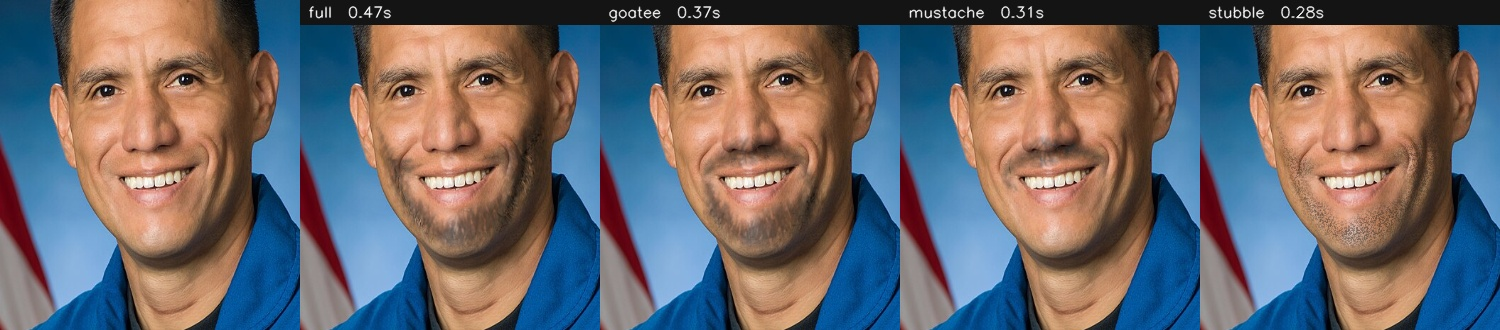
\includegraphics[width=\linewidth]{barba_estilos.jpg}
  \caption{Original y los cuatro estilos de barba sobre un retrato de dominio público: completa, candado, bigote y tres días.}
  \label{fig:barba}
\end{figure}

\subsection{Tinte en CIELAB}
\label{sec:tinte}

El tinte (\archivo{coloring/dye.py}) recibe una máscara suave del pelo $\alpha\in[0,1]$ y un color objetivo con componentes $(L_t,a_t,b_t)$ en CIELAB. La figura~\ref{fig:diag-tinte} resume el proceso.

\begin{figure}[ht]
  \centering
  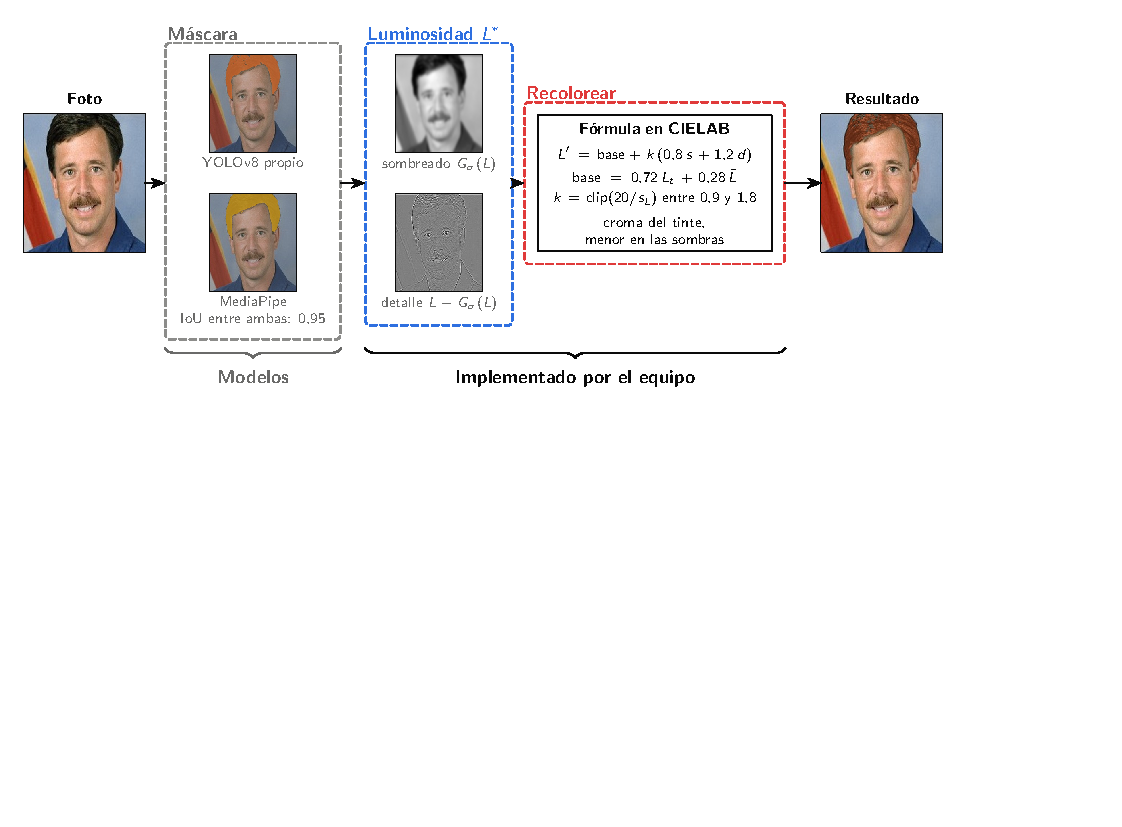
\includegraphics[width=\linewidth]{diagrama_tinte.pdf}
  \caption{Pipeline del tinte: máscara de YOLO o MediaPipe, separación de la luminosidad en sombreado y detalle, y recoloreo en CIELAB.}
  \label{fig:diag-tinte}
\end{figure}


\textbf{Por qué CIELAB.} En una primera versión se cambiaba el tono en HSV. Eso conserva la oscuridad del pelo, así que un pelo negro nunca podía quedar rubio. En CIELAB la luminosidad está separada del color, así que se puede mover la luminosidad base hacia la del tinte sin perder el detalle de cada mechón.

\textbf{Paso 1: luminosidad.} Sean $\bar L$ y $s_L$ la media y la desviación de $L^*$ dentro del pelo, y $G_\sigma$ un desenfoque gaussiano con $\sigma=1{,}5$~px. La imagen se descompone en sombreado (variación lenta) y detalle (mechones):
\begin{align}
  \text{detalle}&=L-G_\sigma(L), & \text{sombreado}&=G_\sigma(L)-\bar L,\\
  L' &= \underbrace{0{,}72\,L_t+0{,}28\,\bar L}_{\text{base}}+k\,(0{,}8\,\text{sombreado}+1{,}2\,\text{detalle}),
  & k&=\operatorname{clip}(20/s_L,\;0{,}9,\;1{,}8).
\end{align}
El factor $k$ normaliza el contraste: un pelo de contraste bajo, como uno negro liso, gana detalle, y uno muy contrastado no se exagera.

\textbf{Paso 2: color.} El croma se toma del tinte y se atenúa en las sombras más profundas, como ocurre con un pigmento real:
\begin{equation}
  a'=128+(a_t-128)\,(0{,}4+0{,}5\,d),\qquad d=\operatorname{clip}\!\left(\frac{L'}{\max(L_t,40)},0,1\right),
\end{equation}
y lo mismo para $b'$.

\textbf{Paso 3: mezcla.} El resultado se mezcla con la imagen original según $\alpha$ multiplicado por la intensidad elegida.

\textbf{Máscara.} La máscara viene de MediaPipe o del YOLO propio (sección~\ref{sec:segmentacion}). Su borde se suaviza hacia adentro, para no teñir la piel ni el fondo.

\subsection{Motor de cortes de pelo}
\label{sec:corte}

El corte es la pieza más compleja de la interfaz de estilos (\archivo{compositing/haircut.py}). Para cortar el pelo hay que resolver cuatro problemas:
\begin{enumerate}
  \item quitar el pelo que sobra y reconstruir lo que había detrás;
  \item saber dónde termina realmente la cabeza;
  \item ubicar la línea del pelo aunque haya flequillo;
  \item hacer crecer pelo corto creíble, con la luz de la foto.
\end{enumerate}
La figura~\ref{fig:diag-corte} muestra las etapas sobre un retrato.

\begin{figure}[ht]
  \centering
  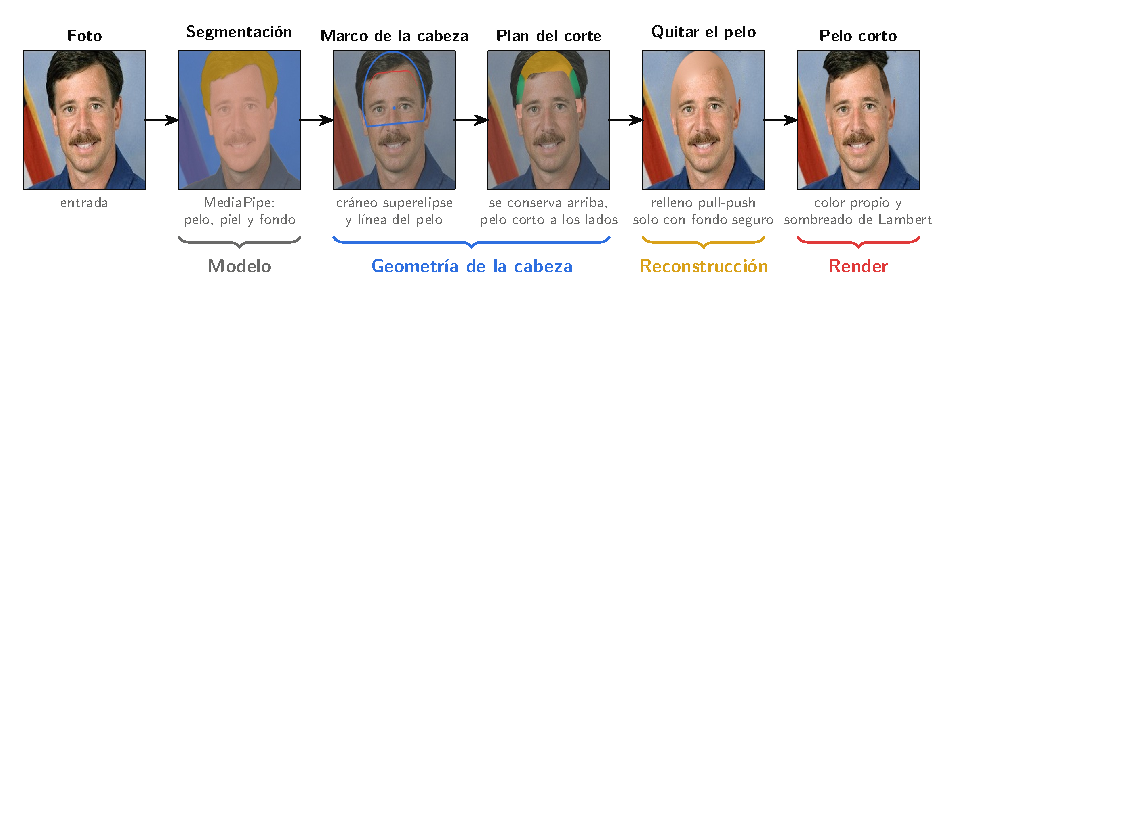
\includegraphics[width=\linewidth]{diagrama_corte.pdf}
  \caption{Pipeline del corte (degradado medio): segmentación, marco de la cabeza con el cráneo y la línea del pelo, plan del corte, relleno con \emph{pull-push} y pelo corto sombreado.}
  \label{fig:diag-corte}
\end{figure}

\textbf{Resolución de trabajo.} El corte se calcula sobre un recorte de la cabeza escalado para que el ancho de la cabeza mida 420~px. Al volver a la resolución original se suma de nuevo el detalle de alta frecuencia de la foto en las zonas que no cambiaron. Así una foto de 4000~px tarda lo mismo que una de 800~px y no pierde nitidez.

\textbf{Línea del pelo.} Primero se busca la frente visible: desde las cejas se sube por la columna central mientras la probabilidad de piel de la cara sea alta.
\begin{itemize}
  \item Si se ven al menos $0{,}2\,w$ de frente, el borde de esa piel es la línea del pelo real.
  \item Si no, hay flequillo, y se asume una frente típica de $0{,}30\,w$ sobre las cejas, en línea con las proporciones faciales de \cite{farkas1994}.
\end{itemize}
Hacia los costados, la línea se retrae un poco en las sienes y baja hasta la patilla con una esquina redondeada (un cuarto de circunferencia). Se le añade un ruido de baja frecuencia para que no sea una línea perfecta.

\textbf{Cráneo.} La cabeza rapada es una superelipse de exponente 2{,}15 en el marco $(x,y)$:
\begin{equation}
  \left|\frac{x}{0{,}55}\right|^{2{,}15}+\left|\frac{\min(y,0)}{y_{\text{tope}}}\right|^{2{,}15}\le1.
\end{equation}
Sus costados bajan hasta las orejas. La altura $y_{\text{tope}}$ se ajusta a cada persona: es la mayor entre la línea del pelo menos $0{,}33\,w$ y la coronilla medida (el punto más alto de pelo o piel en la columna central) más $0{,}03\,w$. Si el pelo ya es corto, el cráneo no sobresale de la silueta real. Por último, el cráneo se intersecta con la silueta de la persona, ligeramente dilatada.

\textbf{Relleno del fondo con \emph{pull-push}.} El pelo que queda fuera del cráneo hay que quitarlo. El primer intento usó \emph{inpainting} de Telea \cite{telea2004}, que propaga el color de todo el borde del hueco; como ese borde incluye pelo, arrastraba el pelo hacia el fondo y dejaba ``pelo fantasma''. La solución es \emph{pull-push} \cite{gortler1996} con una máscara de píxeles conocidos elegida a mano:
\begin{itemize}
  \item cuentan solo los píxeles de fondo seguro ($p_{\text{fondo}}>0{,}6$) o de ropa, fuera del pelo;
  \item cerca del pelo se exige $p_{\text{fondo}}>0{,}9$.
\end{itemize}
En cada nivel de la pirámide, el color es $\sum w\,c/\sum w$, y en la fase \emph{push} se mezcla con el nivel grueso según el peso, $\operatorname{clip}(2w,0,1)$. La figura~\ref{fig:pullpush} compara ambos métodos.

Después del relleno se buscan \textbf{mechones sueltos}: píxeles cerca del hueco que se diferencian del fondo suavizado en más de 30 niveles. Se agregan al hueco y se rellena de nuevo. Además, el fondo rellenado recibe un ruido cuya amplitud es la energía de alta frecuencia local del fondo, propagada también con \emph{pull-push}, para que no se vea más liso que el resto.

\begin{figure}[ht]
  \centering
  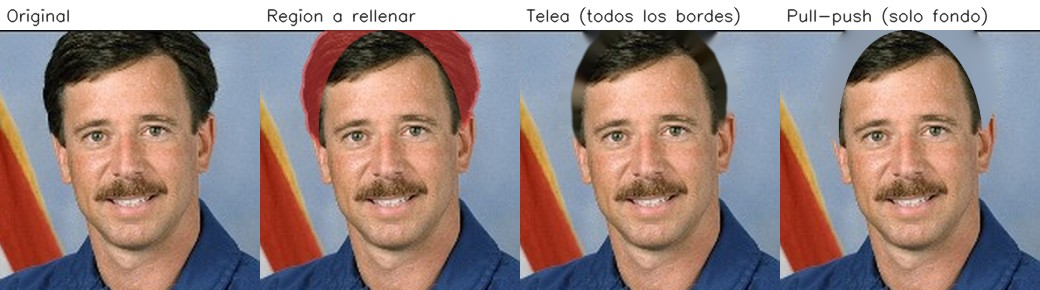
\includegraphics[width=\linewidth]{pull_push.jpg}
  \caption{Rellenar el fondo donde se quita pelo. Telea toma color de todo el borde y arrastra el pelo; \emph{pull-push} con solo píxeles de fondo deja un relleno limpio.}
  \label{fig:pullpush}
\end{figure}

\textbf{Piel bajo el pelo.} Dentro del cráneo, la piel que tapaba el pelo (cuero cabelludo o frente bajo un flequillo) se rellena con \emph{pull-push}. Como fuente se usan solo píxeles de piel de la cara alejados del pelo, porque la piel pegada a la línea del pelo suele estar sombreada y dejaba una marca. La transición hacia la piel real es gradual.

\textbf{Pelo corto.} El pelo nuevo tiene el color del propio pelo: la mediana en CIELAB del 45~\% más oscuro de los píxeles de pelo. Se sombrea con un modelo de Lambert \cite{marschner2016}:
\begin{itemize}
  \item la normal sale de tratar el cráneo como un elipsoide;
  \item la dirección de la luz se estima de la asimetría de brillo entre las dos mitades de la cara, más una componente desde arriba;
  \item la luminosidad final es $L=L_{\text{pelo}}\,(0{,}55+0{,}6\,s)$, donde $s=0{,}62+0{,}38\max(0,\hat n\cdot\hat l)$ es el sombreado.
\end{itemize}
La textura combina dos ruidos: uno anisótropo (desenfoque gaussiano mucho más largo en vertical que en horizontal) que imita trazos cortos, y uno de baja frecuencia para variaciones de densidad. La cobertura del pelo corto es
\begin{equation}
  c = \rho(x,y)\cdot z_{\text{pelo}}\cdot h_{\text{cráneo}}\cdot(1+0{,}08\,n_{\text{trazo}}+0{,}06\,n_{\text{parche}}),
\end{equation}
donde $z_{\text{pelo}}$ vale 1 por encima de la línea del pelo y $\rho$ es la densidad del estilo. La densidad base depende de la intensidad elegida $t$: $\rho_0=0{,}92\,(1{,}1-0{,}4\,t)$. Más intensidad significa pelo más corto, con más cuero cabelludo visible.

\textbf{Estilos.} Todos los cortes se definen sobre el mismo marco. La parte de arriba se conserva dentro de una franja $|x|<r(y)$, con
\begin{equation}
  r(y)=0{,}36+0{,}16\,\operatorname{smoothstep}\!\left(\frac{-0{,}40-y}{0{,}25}\right),
\end{equation}
que se ensancha hacia la coronilla. En los costados, la densidad sube desde la piel en $y_{\text{piel}}$ hasta pelo corto en $y_{\text{corto}}$:
\begin{equation}
  \rho(y)=\rho_0\,\min\!\Big(f+(1-f)\sqrt{\operatorname{smoothstep}\big(\tfrac{y_{\text{piel}}-y}{y_{\text{piel}}-y_{\text{corto}}}\big)},\;c_{\max}\Big),
\end{equation}
donde $f$ es la densidad mínima y $c_{\max}$, la máxima. La tabla~\ref{tab:cortes} da los parámetros.

\begin{table}[ht]
\centering
\small
\begin{tabularx}{\linewidth}{@{}l c c X@{}}
\toprule
Corte & $y_{\text{piel}}$ & $y_{\text{corto}}$ & Particularidad \\
\midrule
Degradado bajo & 0{,}10 & $-0{,}12$ & Piel solo junto a la oreja. \\
Degradado medio & $-0{,}08$ & $-0{,}30$ & Piel hasta la sien. \\
Degradado alto & $-0{,}24$ & $-0{,}46$ & Piel hasta lo alto de los costados. \\
\emph{Taper} & 0{,}24 & 0{,}00 & Nunca llega a piel: $f=0{,}35$. \\
\emph{Undercut} & -- & -- & Costados planos y muy cortos ($c_{\max}=0{,}22$) con borde duro (transición de $0{,}02\,w$). \\
Raya marcada & $-0{,}08$ & $-0{,}30$ & Degradado medio más una línea afeitada en $x=r(y)-0{,}09$ sobre el cuero cabelludo de un lado. \\
\emph{Crew cut} & -- & -- & Todo corto, más denso arriba; conserva el 30~\% de la textura original arriba y sube el tope del cráneo $0{,}035\,w$. \\
Rapado & -- & -- & Pelo corto uniforme por encima de la línea del pelo. \\
\bottomrule
\end{tabularx}
\caption{Parámetros de cada corte en el marco de la cabeza (unidades de ancho de cabeza, $y$ hacia abajo).}
\label{tab:cortes}
\end{table}

\textbf{Protección de la cara.} El polígono de la cara, contraído un 5~\% hacia su centro y erosionado, nunca se modifica; las pruebas automáticas lo verifican para los ocho cortes. La contracción deja libres las patillas del borde, que se degradan junto con los costados.

\subsection{Tinte también en la barba}
\label{sec:barbatinte}

Para teñir la barba hay que encontrarla, y el segmentador no la marca como pelo. \archivo{segmentation/facial_hair.py} trabaja dentro de la zona donde crece una barba completa, recortada en el borde de la mandíbula. Un píxel cuenta como barba si cumple tres condiciones:
\begin{enumerate}
  \item es \textbf{más oscuro} que la piel de la propia persona: $\operatorname{smoothstep}((L_{\text{piel}}-L-10)/25)$, donde $L_{\text{piel}}$ se mide en las mejillas, sobre la nariz;
  \item tiene \textbf{textura de pelo}: desviación local de $L$ alta en una ventana de $0{,}012\,w$;
  \item es \textbf{menos rojo} que la piel, porque el pelo tiene menos $a^*$.
\end{enumerate}
Las sombras lisas no cumplen la condición de textura. El borde largo de la mandíbula sí la cumple, pero se descarta con la coherencia del tensor de estructura \cite{bigun1987}: un borde recto tiene coherencia cercana a 1, mientras que la barba tiene trazos en todas direcciones. Finalmente, las zonas oscuras encerradas por barba detectada (el centro de un candado negro, que no tiene textura) se incorporan con un cierre morfológico.

Probado sobre 10 caras, las cinco sin barba quedan limpias y los bigotes se detectan completos. Cuando la barba la puso la propia aplicación (sección~\ref{sec:combinar}), su estilo se conoce y se usa directamente la máscara de ese estilo.

\subsection{Combinación de looks y ficha para el barbero}
\label{sec:combinar}

Bajo cada resultado, la interfaz ofrece aplicar otra herramienta sobre él. Por ejemplo:
\begin{enumerate}
  \item primero la barba;
  \item luego el tinte con barba;
  \item al final el corte (figura~\ref{fig:combinado}).
\end{enumerate}
El resultado de cada paso pasa a ser la foto de la herramienta siguiente. El comparador sigue mostrando la foto original como ``antes''. El tinte, al recibir una foto con barba hecha por la aplicación, recibe también el estilo de esa barba. El corte toma el color del pelo ya teñido.

El look guardado lleva el nombre de todos los pasos. La ficha para el barbero (figura~\ref{fig:ficha}) lista cada servicio con una indicación práctica:
\begin{itemize}
  \item el número de máquina o de peine;
  \item dónde va cada número;
  \item la referencia hexadecimal del color.
\end{itemize}

\begin{figure}[ht]
  \centering
  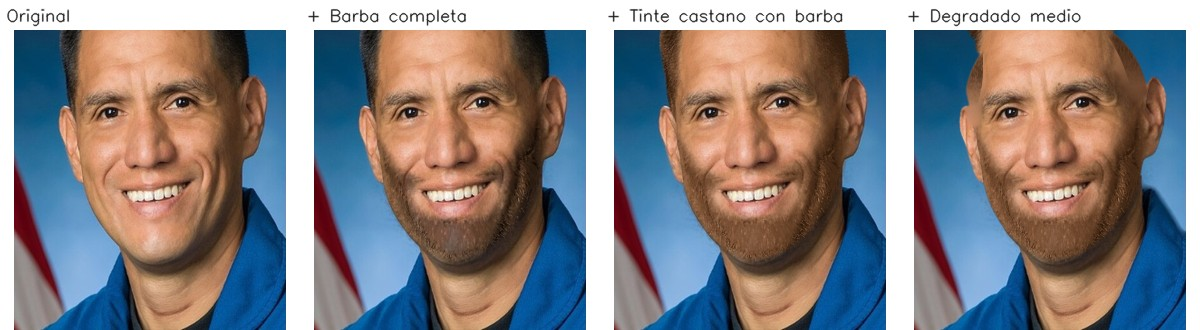
\includegraphics[width=\linewidth]{combinado.jpg}
  \caption{Look combinado sobre el retrato de ejemplo: barba completa, tinte castaño que incluye la barba y degradado medio.}
  \label{fig:combinado}
\end{figure}

\subsection{Física de la barba}
\label{sec:fisica}

En el modo en vivo, la barba larga se simula con física (\archivo{compositing/beard_physics.py}).

\textbf{Modelo.} Cada hebra es una cadena de cuatro partículas, y hay una hebra por cada 30 píxeles de la región (hasta 2600):
\begin{itemize}
  \item la raíz se guarda en coordenadas baricéntricas de la malla de referencia, así que sigue a la piel en cada cuadro;
  \item la pose de reposo crece en la dirección del pelo y gira con la cabeza;
  \item el largo depende de cuánto está la raíz por debajo de la boca;
  \item las raíces del labio superior crecen hacia los costados, para que no cuelguen sobre los dientes.
\end{itemize}

\textbf{Integración.} En cada cuadro se dan cuatro subpasos de longitud $h=\Delta t/4$ con Verlet amortiguado \cite{verlet1967}:
\begin{align}
  v &= 0{,}86\,(x-x_{\text{prev}}), & x &\leftarrow x+v+g\,h^2, & x &\leftarrow x+k_i\,(x_{\text{reposo}}-x),
\end{align}
con $g=2{,}2\,w$~px/s² y una rigidez $k_i=[0;\,0{,}34;\,0{,}22;\,0{,}13]$ que baja hacia la punta: la base sigue a la cara y la punta tiene inercia. Después, dos iteraciones de restricción de distancia (PBD \cite{jakobsen2001,muller2007}) mantienen el largo de cada tramo. Por eso la hebra se balancea como un péndulo y no se estira. La raíz se interpola entre el cuadro anterior y el actual para que no salte.

\textbf{Render.} Cada hebra se suaviza con un corte de esquinas de Chaikin \cite{chaikin1974}, de 4 a 8 puntos. Cada tramo se dibuja como una gaussiana 2D alargada, con $\sigma$ a lo largo igual a medio tramo y de 0{,}5 a 0{,}75~px a lo ancho. Las gaussianas se acumulan sin ordenar, con densidad $A=\sum o_iG_i$ y cobertura $\alpha=1-e^{-A}$, como en la ley de Beer--Lambert, de modo que muchos pelos superpuestos saturan suavemente. Unos 2000 tramos cuestan unos 10~ms, vectorizados sobre parches de $13\times13$.

En una secuencia con vaivén y un tirón brusco, el retraso de las puntas llega a entre 8 y 12~px y se recupera solo. La correlación entre la velocidad de la cabeza y el retraso es de 0{,}78 a 0{,}82 (figura~\ref{fig:fisica}).

\begin{figure}[ht]
  \centering
  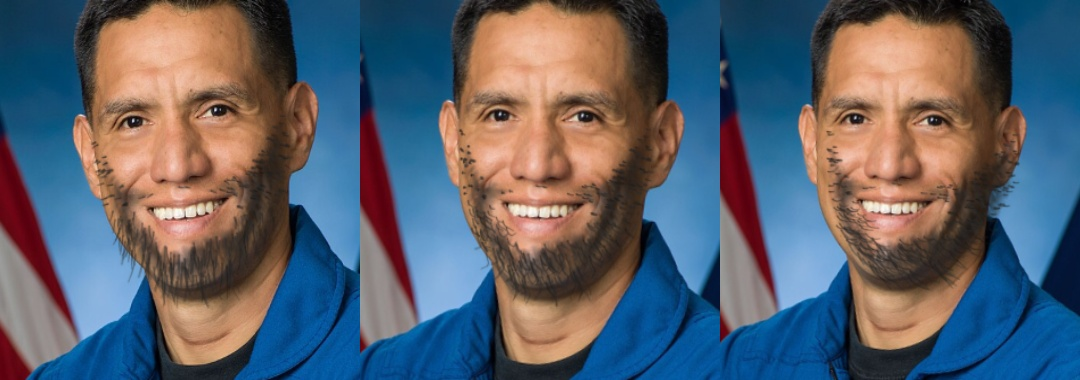
\includegraphics[width=0.85\linewidth]{fisica.jpg}
  \caption{Barba con física: en reposo y durante un movimiento rápido de la cabeza. Las puntas se atrasan y luego vuelven.}
  \label{fig:fisica}
\end{figure}

\subsection{Gaussianas 2D: ``¿Cuántas gaussianas eres?''}
\label{sec:gauss2d}

\archivo{splatting/gaussian_image.py} reconstruye un retrato con $N$ gaussianas 2D, al estilo de GaussianImage \cite{zhang2024}, sin bibliotecas de diferenciación automática.

\textbf{Representación.} Cada gaussiana tiene un centro $\mu_i$, un peso RGB $c_i$ y el factor de Cholesky de la inversa de su covarianza, $L=\begin{psmallmatrix}l_1&0\\l_2&l_3\end{psmallmatrix}$. Con $\Sigma^{-1}=LL^\top$, la covarianza es siempre definida positiva. Con $u=l_1d_x+l_2d_y$ y $v=l_3d_y$:
\begin{equation}
  G_i(x)=\exp\!\big(-\tfrac12(u^2+v^2)\big),\qquad C(x)=\sum_i c_i\,G_i(x).
\end{equation}

\textbf{Optimización.} Se minimiza el error cuadrático medio contra la imagen, usando gradientes analíticos:
\begin{itemize}
  \item respecto de la forma: $\partial q/\partial l_1=2u\,d_x$, $\partial q/\partial l_2=2u\,d_y$ y $\partial q/\partial l_3=2v\,d_y$;
  \item respecto del centro: $\partial q/\partial\mu_x=-2u\,l_1$ y $\partial q/\partial\mu_y=-2u\,l_2-2v\,l_3$.
\end{itemize}
Los parámetros se actualizan con Adam \cite{kingma2015} escrito a mano, en 110 a 160 iteraciones.

\textbf{Detalles de implementación.}
\begin{itemize}
  \item La inicialización coloca más gaussianas donde hay bordes: muestrea con probabilidad proporcional a $0{,}35+|\nabla I|$.
  \item Cada gaussiana se evalúa solo en un parche de radio $\lceil2{,}5\,\sigma_{\max}\rceil$, y los parches se agrupan por radio. Así no hay bucles por gaussiana.
  \item La acumulación usa \texttt{np.bincount}. Una etapa pasó de 10--21~s a 1--4~s.
\end{itemize}

La interfaz lo convierte en un juego: el retrato aparece con 20, 60, 200, 600 y 2000 gaussianas, y hay que reconocer la cara lo antes posible (figura~\ref{fig:gauss2d}).

\begin{figure}[ht]
  \centering
  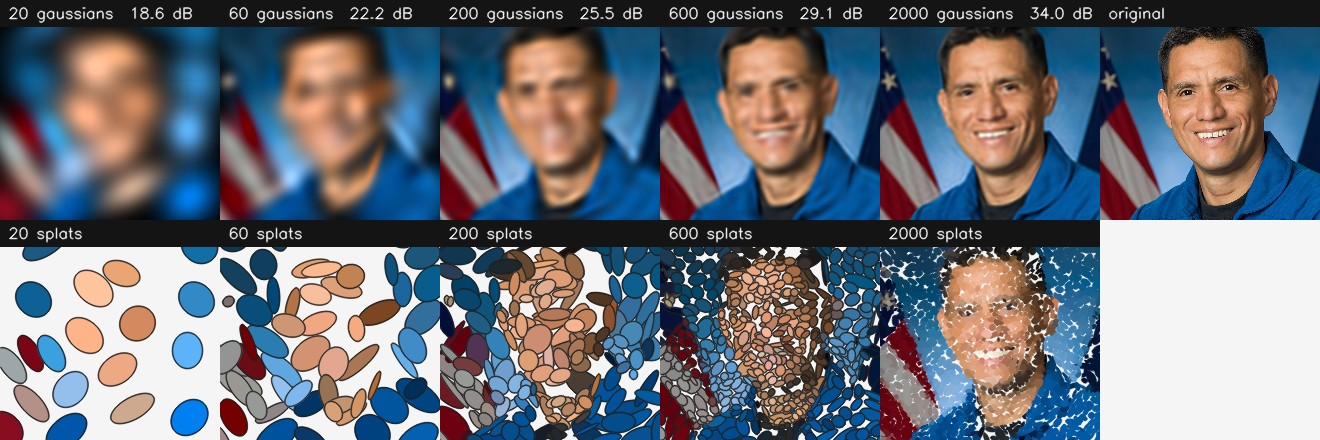
\includegraphics[width=\linewidth]{gaussianas2d.jpg}
  \caption{Retrato reconstruido con 20, 60, 200, 600 y 2000 gaussianas 2D junto al original (arriba), y cada gaussiana dibujada como una elipse (abajo).}
  \label{fig:gauss2d}
\end{figure}

\subsection{Espejo 3D con \emph{Gaussian Splatting}}
\label{sec:espejo}

El espejo convierte una foto en una cabeza de unas 100\,000 gaussianas 3D que se puede girar. Implementa, desde cero, el paso de \emph{render} de 3DGS \cite{kerbl2023}. Las gaussianas no se entrenan desde varias vistas: se construyen a partir de una sola foto y de la malla 3D de MediaPipe.

\textbf{Construcción} (\archivo{splatting/head3d.py}).
\begin{enumerate}
  \item La malla de 478 puntos se triangula con el Delaunay propio en $(x,y)$ y se eleva a 3D con la profundidad estimada.
  \item \textbf{Cara}: cada triángulo recibe gaussianas en proporción a su área 3D (no a la proyectada), con muestreo estratificado. Cada gaussiana es un disco tangente, $\Sigma=R\operatorname{diag}(s^2,s^2,(0{,}4s)^2)R^\top$, donde $R$ es el marco del triángulo. Su color se lee de la foto con interpolación bilineal.
  \item \textbf{Barba}: cada hebra son tres gaussianas alargadas que crecen hacia afuera y hacia abajo desde raíces ancladas con coordenadas baricéntricas.
  \item \textbf{Resto de la foto} (pelo, orejas, fondo): un relieve cuya profundidad se acerca a la del contorno de la cara más cercano, con caída exponencial.
\end{enumerate}

\textbf{Visor} (\archivo{frontend/js/splat3d.js}, WebGL2). Para cada gaussiana:
\begin{itemize}
  \item el \emph{vertex shader} proyecta la covarianza con EWA, $\Sigma_{2D}=JW\Sigma W^\top J^\top+0{,}3\,I$ \cite{zwicker2001}, calcula autovalores y autovectores en forma cerrada y dibuja un cuadrilátero orientado de $\pm3\sigma$;
  \item el \emph{fragment shader} evalúa $\alpha=a\,e^{-r^2/2}$.
\end{itemize}
Las gaussianas se ordenan de atrás hacia adelante con un \emph{counting sort} de 16 bits, en tiempo $O(N)$, y se mezclan con \texttt{SRC\_ALPHA, ONE\_MINUS\_SRC\_ALPHA}. La opción ``Ver cada gaussiana'' achica la huella para mostrar la técnica (figura~\ref{fig:espejo}).

\textbf{Exportación.} Se exporta al formato \texttt{.ply} de 3DGS, compatible con visores externos:
\begin{itemize}
  \item la covarianza se descompone en escala y cuaternión;
  \item el color pasa a armónicos esféricos de grado 0, $f=(c-0{,}5)/0{,}2821$;
  \item la opacidad pasa a \emph{logit}.
\end{itemize}

\begin{figure}[ht]
  \centering
  \begin{subfigure}{0.32\linewidth}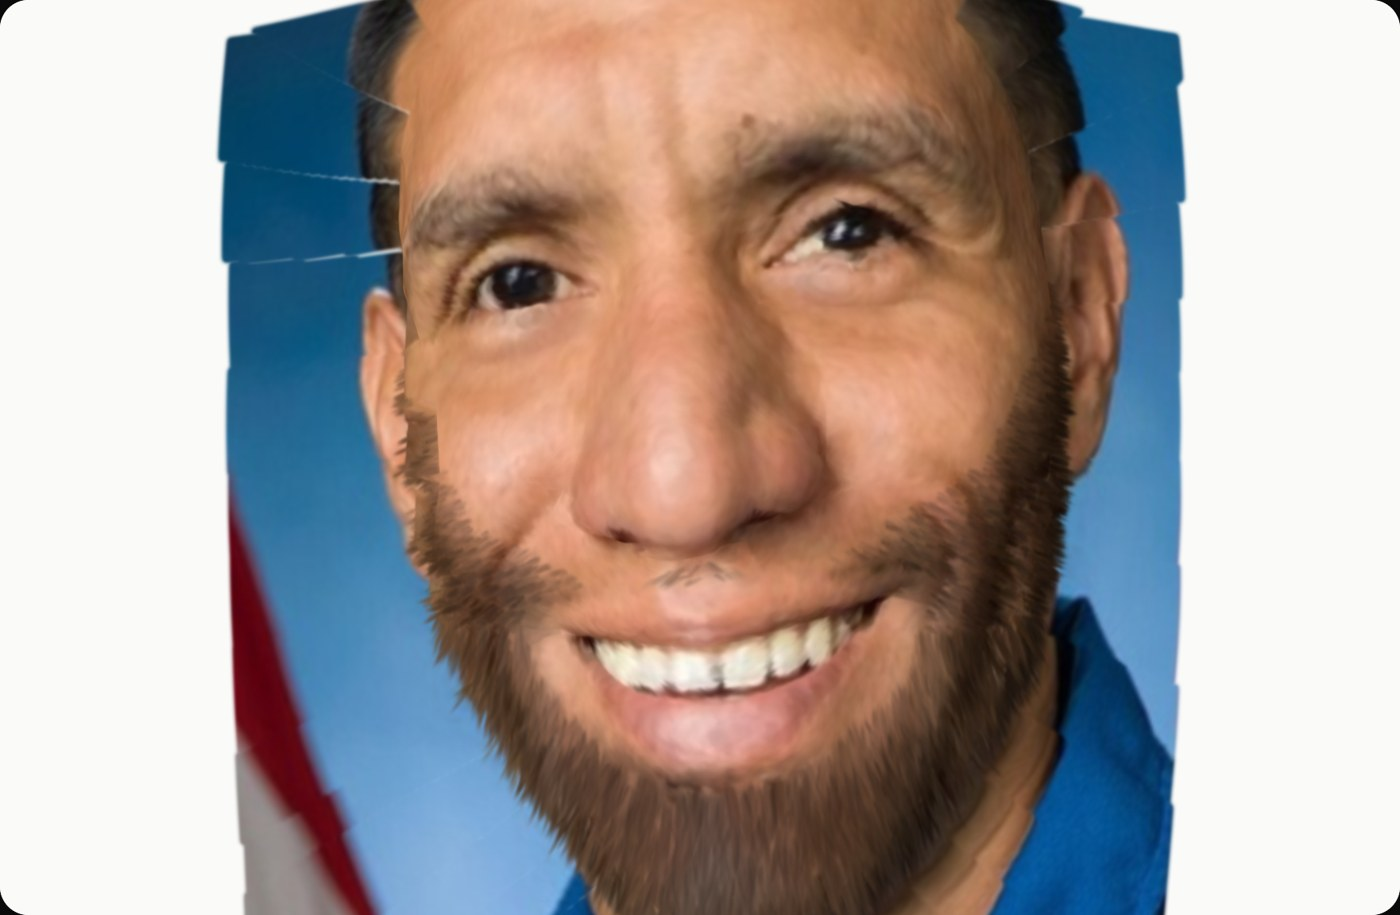
\includegraphics[width=\linewidth]{espejo3d_frente.jpg}\caption{Frente}\end{subfigure}\hfill
  \begin{subfigure}{0.32\linewidth}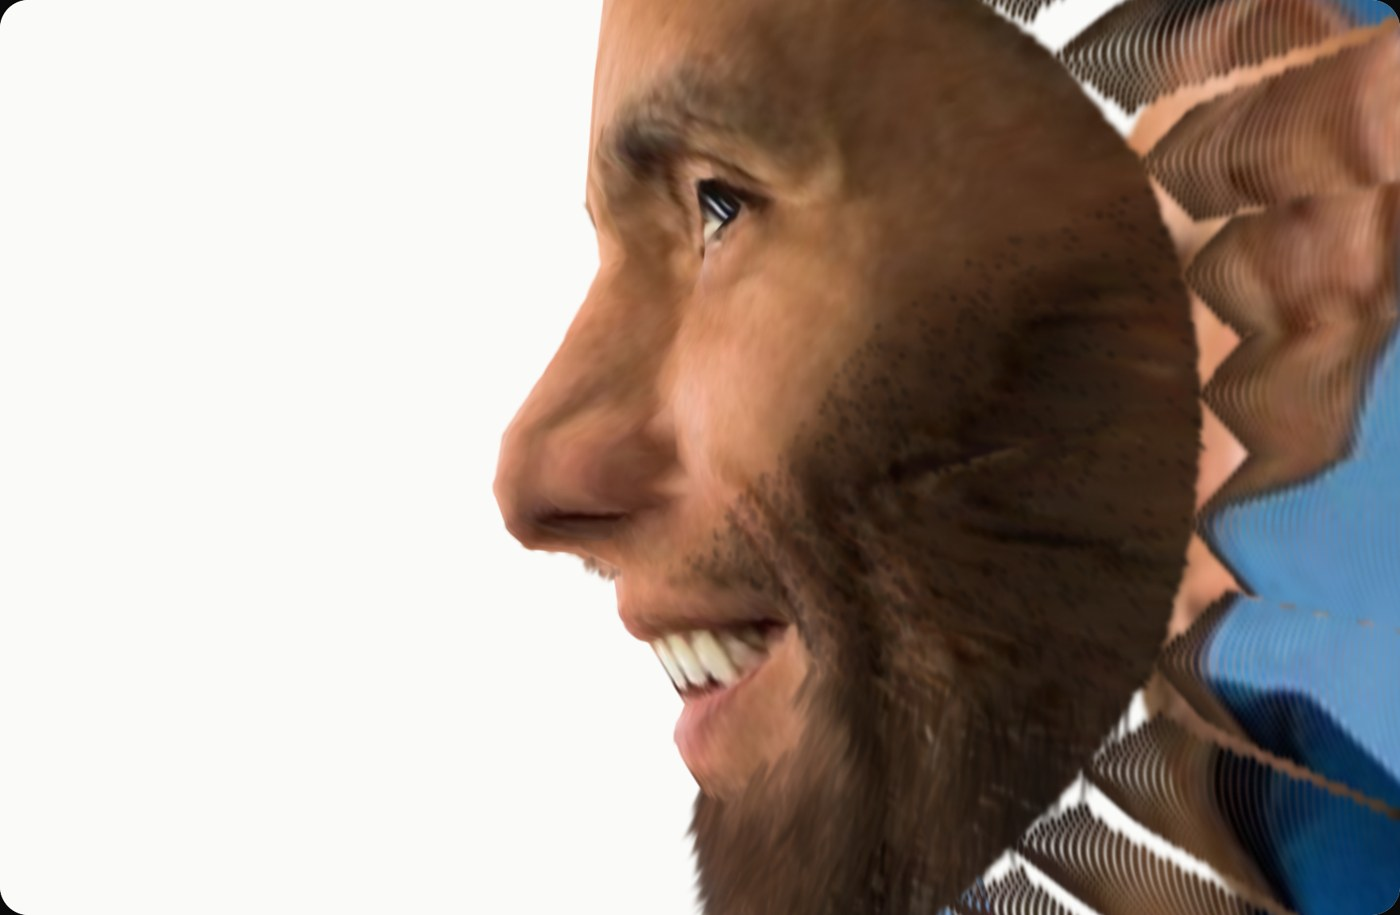
\includegraphics[width=\linewidth]{espejo3d_giro.jpg}\caption{Girada}\end{subfigure}\hfill
  \begin{subfigure}{0.32\linewidth}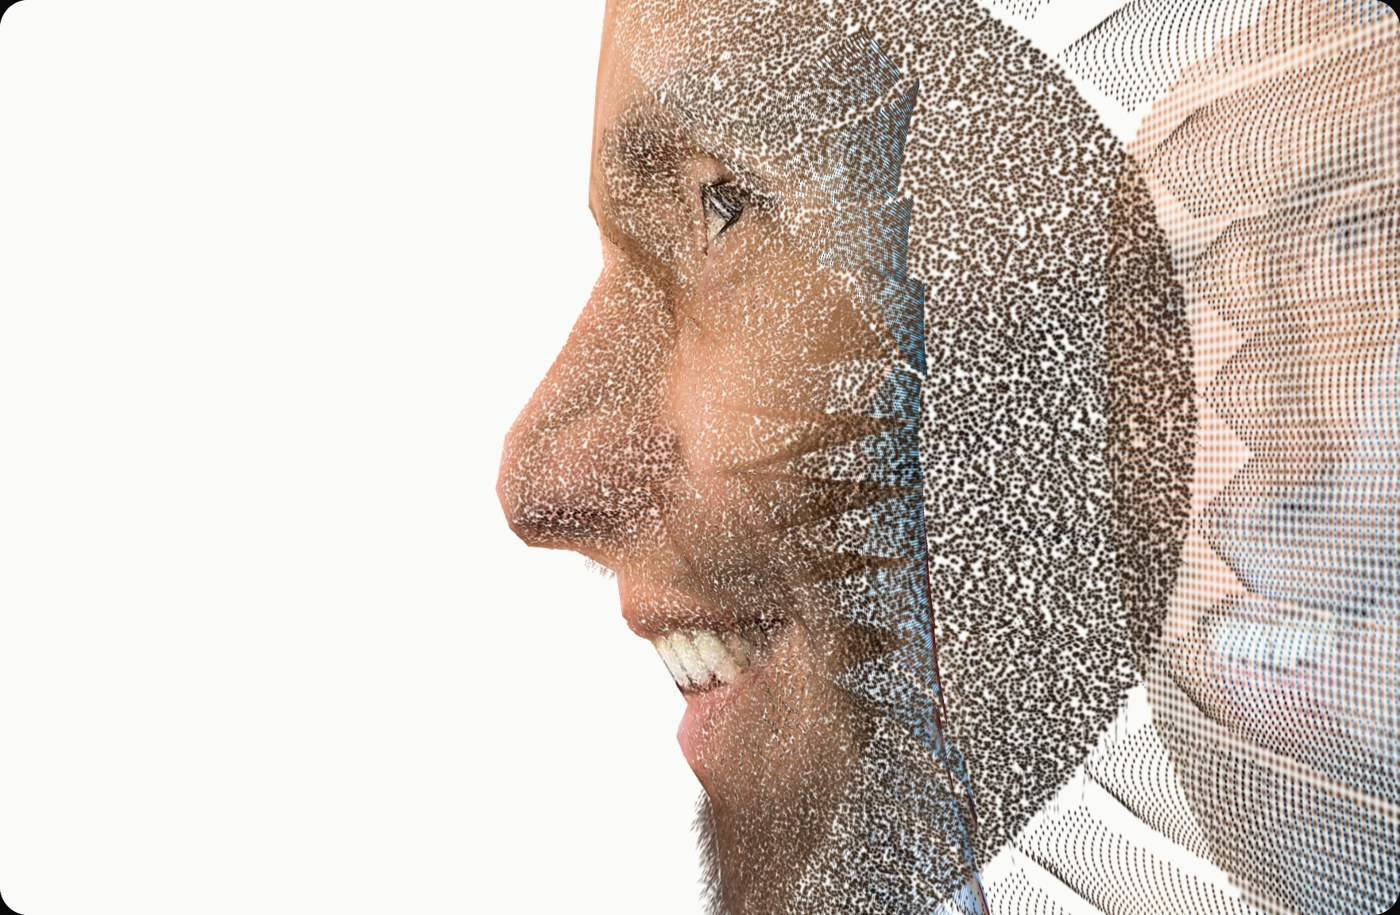
\includegraphics[width=\linewidth]{espejo3d_splats.jpg}\caption{Cada gaussiana}\end{subfigure}
  \caption{Espejo 3D con barba completa, construido desde una sola foto. Al girar mucho se ven los límites de reconstruir desde una vista: el relieve detrás de la cara se estira.}
  \label{fig:espejo}
\end{figure}

\subsection{Peluca 3D multivista}
\label{sec:peluca}

La peluca 3D escanea el peinado de una persona con la cámara y lo convierte en una peluca de gaussianas. Esa peluca se puede ver sobre un maniquí, sobre la cara escaneada o sobre otra persona en vivo (\archivo{splatting/hair3d.py}, \archivo{splatting/face3d.py}, \archivo{compositing/bald.py}).

\textbf{Escaneo.} Durante 12 segundos la persona gira la cabeza unos 180°, y se guardan capturas con el ángulo de giro estimado. En cada captura, la máscara de pelo se obtiene combinando el segmentador, la distancia de color al pelo y una elipse de la cabeza (\archivo{segmentation/transfer_mask.py}).

\textbf{Forma: \emph{visual hull} por cortes.} Para cada altura y cada dirección horizontal (360 direcciones), cada captura indica, desde su ángulo, dónde empieza y dónde termina el pelo. Intersecar esas franjas da el corte transversal real de la peluca, es decir, la envolvente visual \cite{laurentini1994}, calculada rebanada por rebanada. Las direcciones que ninguna captura vio siguen una forma de cabeza:
\begin{itemize}
  \item tan ancha como la vista más frontal;
  \item nunca delante de la cara;
  \item redondeada sobre el cráneo y más plana donde cuelga pelo largo.
\end{itemize}

\textbf{Textura.} Cada punto de la superficie toma color de las capturas que mejor lo ven, mezcladas según qué tan de frente lo ven, para que no haya costuras. La nuca nunca se ve: recibe el color del último pelo que vio cada perfil, con estrías verticales. Cada gaussiana se alarga en la dirección del pelo, estimada con el tensor de estructura (perpendicular al gradiente dominante; hacia abajo donde no hay orientación clara).

\textbf{Estudio.} En el navegador, la peluca se puede editar de tres formas:
\begin{itemize}
  \item \textbf{color}: se recolorean las gaussianas con la intensidad elegida;
  \item \textbf{largo}: se eliminan las gaussianas por debajo de una altura;
  \item \textbf{tijeras}: un pincel en pantalla corta las gaussianas más cercanas a la cámara dentro de su radio, usando la proyección de cada gaussiana; los cortes se pueden deshacer.
\end{itemize}

\textbf{Prueba en vivo.} Para probar la peluca sobre otra persona, el navegador sigue la cabeza con MediaPipe en JavaScript y el servidor quita el pelo propio de esa persona. El fondo se aprende de cuadros anteriores o se rellena, y el cuero cabelludo se sombrea a partir de la piel de la cara. La figura~\ref{fig:peluca} muestra una peluca construida desde una sola foto, el caso mínimo; con el escaneo de 180° se cierra también la parte de atrás.

\begin{figure}[ht]
  \centering
  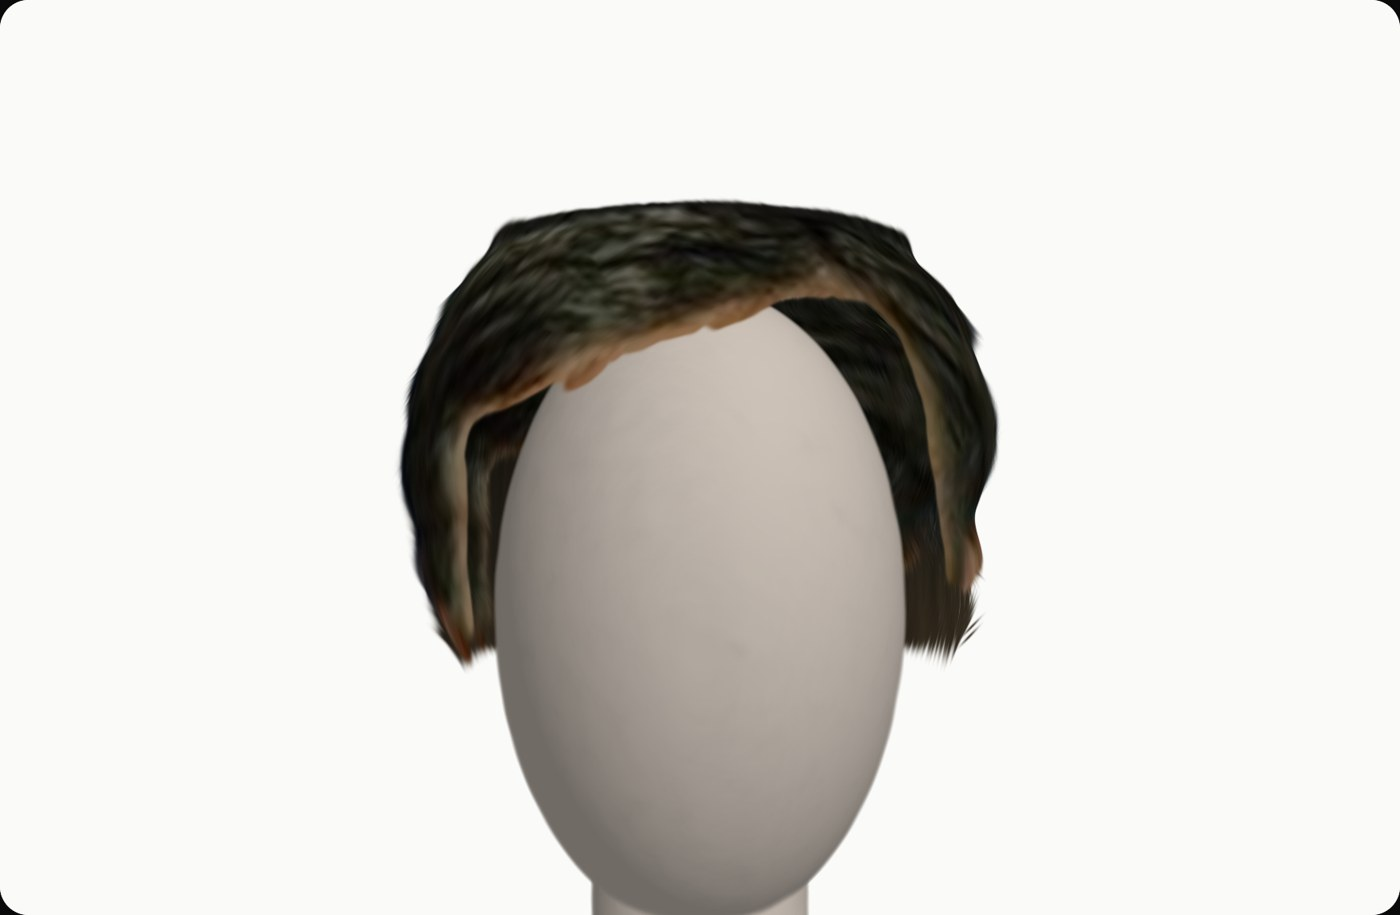
\includegraphics[width=0.55\linewidth]{peluca3d.jpg}
  \caption{Peluca de gaussianas sobre el maniquí, construida desde un único retrato frontal.}
  \label{fig:peluca}
\end{figure}

\subsection{Laboratorio: avatar en vivo}
\label{sec:lab}

El laboratorio (\archivo{lab/avatar.py}) escanea la cabeza desde varios ángulos y construye un avatar de gaussianas. Cada gaussiana guarda su triángulo de la malla, sus coordenadas baricéntricas, un desplazamiento y una covarianza expresados en el marco local del triángulo. Ese marco es ortonormal: $e_1$ es la primera arista normalizada, $n$ la normal y $e_2=n\times e_1$. Con $R=[e_1\;e_2\;n]$ y $s$ el ancho de la cara, la covarianza en el mundo es $R\,\Sigma_{\text{local}}\,R^\top s^2$.

En cada cuadro de la cámara, la malla nueva reconstruye el marco de cada triángulo y la gaussiana lo sigue. Por eso el avatar copia los gestos de la persona y puede verse de perfil. Está marcado como experimental en la interfaz.

\subsection{Contrarreloj: el juego de afeitado}
\label{sec:juego}

La persona tiene 30 segundos para afeitar una barba con física hasta dejar un estilo objetivo: candado, bigote o collar (\archivo{game/speedrun.py}). La ``máquina'' puede ser el mouse o la punta del dedo índice, detectada con el modelo de mano de MediaPipe; corta solo con el índice extendido y el dedo medio doblado.

\textbf{Detección del corte.} A 10~cuadros por segundo, el dedo salta decenas de píxeles entre cuadros, así que probar si toca un punto dejaría pelos sin cortar. En su lugar, se cortan las hebras cuya raíz o primer nodo está a menos de $r=0{,}05\,w$ del segmento recorrido $\overline{p_0p_1}$:
\begin{equation}
  t=\operatorname{clamp}\!\left(\frac{(x-p_0)\cdot(p_1-p_0)}{\lVert p_1-p_0\rVert^2},0,1\right),\qquad d=\lVert x-(p_0+t(p_1-p_0))\rVert.
\end{equation}
Las hebras cortadas caen con física y se desvanecen.

\textbf{Puntaje.} Se calcula como
\begin{equation}
  1000\cdot\text{limpieza}\cdot\text{conservación},
\end{equation}
donde la limpieza es la fracción de pelo afeitado fuera del objetivo y la conservación, la fracción de pelo que queda dentro de él. Se descartó la IoU como puntaje porque, sin tocar nada, ya daba 0{,}72 para el candado.

\begin{figure}[ht]
  \centering
  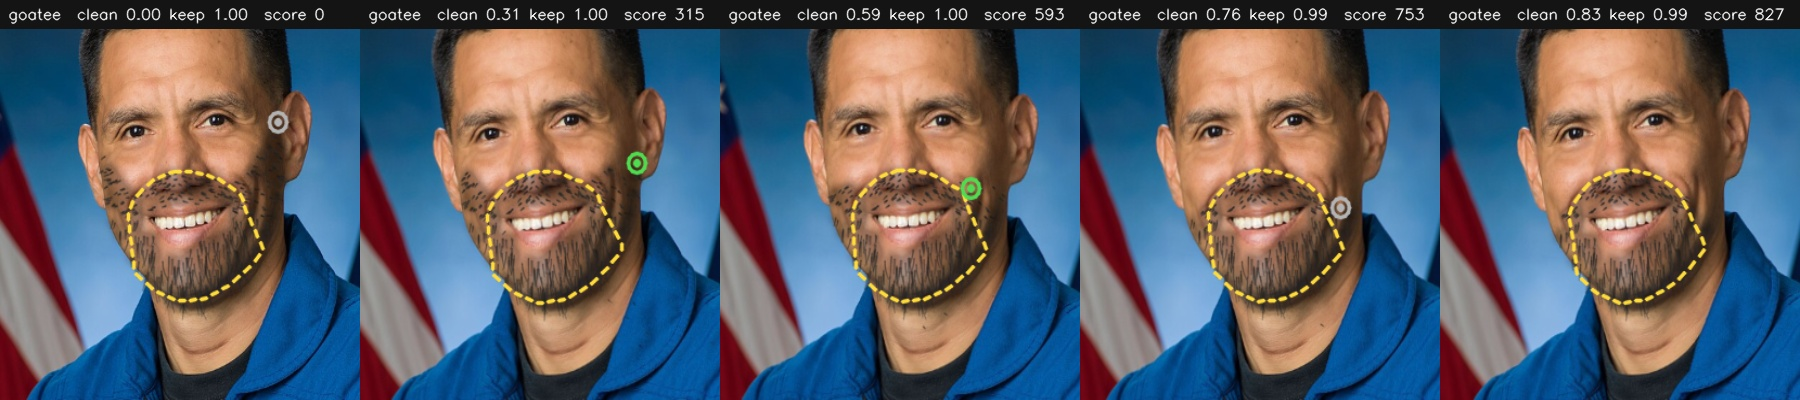
\includegraphics[width=\linewidth]{contrarreloj.jpg}
  \caption{Una ronda de Contrarreloj con objetivo ``candado'', de la barba completa al estilo final.}
  \label{fig:juego}
\end{figure}


\section{Herramientas utilizadas}
\label{sec:herramientas}

La tabla~\ref{tab:herramientas} indica qué herramienta resolvió cada parte del proyecto. Donde dice ``propio'', el algoritmo está escrito por el equipo sobre operaciones básicas de NumPy.

\begin{table}[ht]
\centering
\small
\begin{tabularx}{\linewidth}{@{}l X@{}}
\toprule
Herramienta & Qué resolvió \\
\midrule
Python 3.12 + NumPy \cite{harris2020} & Lenguaje del servidor y operaciones vectorizadas sobre imágenes. Base de todos los algoritmos propios. \\
FastAPI \cite{fastapi} + Uvicorn & Servidor HTTP y API; también sirve la interfaz web. \\
OpenCV \cite{bradski2000} & Lectura y escritura de imágenes, conversiones de color, desenfoques, morfología, \emph{distance transform}, clasificador de Haar, filtro guiado e \emph{inpainting} de Telea (solo como referencia de comparación). \\
MediaPipe \cite{lugaresi2019} & Modelos preentrenados, usados solo para inferencia: malla facial de 478 puntos, segmentador multiclase y puntos de la mano. También corre en el navegador para seguir la cabeza en la prueba en vivo de la peluca. \\
Ultralytics YOLOv8 + PyTorch \cite{jocher2023,paszke2019} & Ajuste fino y ejecución del segmentador de pelo propio (\archivo{hair_best.pt}). Es opcional: sin él, la aplicación usa MediaPipe. \\
Google Colab & Entrenamiento de YOLO con GPU (\archivo{backend/training/barberstudio_colab.ipynb}). \\
WebGL2 \cite{khronos2017} & Visor de gaussianas 3D en el navegador (\emph{shaders} propios). \\
HTML, CSS y JavaScript nativos & Interfaz sin \emph{frameworks} ni compilación. \\
pytest + GitHub Actions & 53 pruebas automáticas que se ejecutan en cada cambio. \\
Docker & Imagen reproducible con todas las dependencias y los modelos. \\
\LaTeX{} & Este documento. \\
\bottomrule
\end{tabularx}
\caption{Herramientas y la parte del proyecto que resolvió cada una.}
\label{tab:herramientas}
\end{table}

\begin{table}[ht]
\centering
\small
\begin{tabularx}{\linewidth}{@{}X l@{}}
\toprule
Pieza & Origen \\
\midrule
Detección de cara (Haar), 478 puntos faciales, segmentación base, puntos de la mano & Biblioteca o modelo \\
Segmentador de pelo YOLOv8 & Arquitectura de biblioteca, ajuste fino propio \\
Triangulación de Delaunay (Fortune y Bowyer--Watson) & Propio \\
\emph{Warp} afín, coordenadas baricéntricas, interpolación bilineal & Propio \\
Composición de la barba, hebras, \emph{feather}, anclaje a la malla & Propio \\
Tinte en CIELAB, tinte de barba, forma de la cara & Propio \\
Motor de cortes (\emph{pull-push}, cráneo, línea del pelo, sombreado) & Propio \\
Física de hebras (Verlet + PBD) y juego & Propio \\
Gaussianas 2D (gradientes analíticos, Adam) & Propio \\
Gaussianas 3D, proyección EWA, ordenamiento, exportación \texttt{.ply} & Propio \\
Peluca multivista (\emph{visual hull} por cortes, textura, estudio) & Propio \\
\bottomrule
\end{tabularx}
\caption{Qué viene de bibliotecas y qué implementó el equipo.}
\label{tab:propio}
\end{table}

Los efectos animados de la interfaz (texto que rota, títulos que aparecen, franja de líneas) son versiones en JavaScript nativo de componentes de React Bits, con licencia MIT y \emph{Commons Clause}. Los retratos de prueba de las figuras son retratos oficiales de la NASA, de dominio público.

\section{Cómo reproducir el proyecto}
\label{sec:reproduccion}

Esta sección permite instalar y ejecutar Fresh desde cero. El código fuente completo se entrega en la carpeta \archivo{codigo-fuente/}, que contiene lo mismo que la raíz del repositorio. Los comandos se escriben en una terminal (macOS, Linux o Windows con WSL), situada en esa carpeta.

\subsection{Opción A: con Docker (recomendada)}

Es la forma más simple, porque instala todas las dependencias y los modelos dentro de un contenedor.
\begin{enumerate}
  \item Instalar Docker Desktop desde \texttt{https://www.docker.com} y abrirlo.
  \item Construir la imagen y levantar la aplicación (la primera vez tarda varios minutos porque descarga PyTorch):
\begin{lstlisting}
docker compose up -d --build app
\end{lstlisting}
  \item Esperar a que el contenedor esté sano y abrir \texttt{http://localhost:8000} en Chrome:
\begin{lstlisting}
docker compose ps
\end{lstlisting}
  \item Para detenerla:
\begin{lstlisting}
docker compose down
\end{lstlisting}
\end{enumerate}

\subsection{Opción B: con Python}

\begin{enumerate}
  \item Instalar Python 3.12 desde \texttt{https://www.python.org}.
  \item Crear un entorno virtual e instalar las dependencias:
\begin{lstlisting}
cd backend
python3 -m venv venv
source venv/bin/activate
pip install -r requirements.txt -r requirements-dev.txt
\end{lstlisting}
  \item Opcional, para usar el YOLO propio:
\begin{lstlisting}
pip install -r requirements-yolo.txt
pip uninstall -y opencv-python
pip install --force-reinstall --no-deps "opencv-contrib-python>=4.9,<5"
\end{lstlisting}
  Ultralytics instala \texttt{opencv-python}, que pisa a \texttt{opencv-contrib-python} y elimina los módulos \texttt{cv2.face} y \texttt{cv2.ximgproc}. Las dos últimas líneas lo corrigen.
  \item Iniciar el servidor desde la carpeta \archivo{backend}:
\begin{lstlisting}
uvicorn app.main:app --port 8000
\end{lstlisting}
  O, desde la raíz, \texttt{./run.sh}, que hace los pasos 2 y 4 automáticamente.
  \item Abrir \texttt{http://localhost:8000}.
\end{enumerate}

\subsection{Modelos}

Todos los modelos necesarios están en \archivo{backend/models/}:
\begin{itemize}
  \item \archivo{face_landmarker.task}: malla facial de MediaPipe.
  \item \archivo{selfie_multiclass_256x256.tflite}: segmentador multiclase de MediaPipe.
  \item \archivo{hand_landmarker.task}: puntos de la mano, para el juego.
  \item \archivo{lbfmodel.yaml}: puntos de respaldo de OpenCV.
  \item \archivo{hair_best.pt}: el YOLO de pelo entrenado por el equipo.
\end{itemize}
Si falta \archivo{hair_best.pt} o no está instalado Ultralytics, la aplicación usa MediaPipe y el selector de modelo no aparece. La interfaz carga dos recursos desde internet: las fuentes tipográficas, que tienen respaldo local si no cargan, y la versión en JavaScript de MediaPipe, que solo usa la prueba en vivo de la peluca.

\subsection{Pruebas}

Desde \archivo{backend}, con el entorno activado:
\begin{lstlisting}
python -m pytest tests -q
\end{lstlisting}
El resultado esperado es \texttt{54 passed}.

\subsection{Reentrenar el segmentador de pelo}

\begin{enumerate}
  \item Descargar Figaro1k \cite{svanera2016} y CelebAMask-HQ \cite{lee2020} en \archivo{data/}. Las páginas de los datasets indican cómo pedir acceso; no se incluyen por tamaño y licencia.
  \item Convertir las máscaras a polígonos de YOLO:
\begin{lstlisting}
python backend/training/prepare_hair_dataset.py
\end{lstlisting}
  \item Abrir \archivo{backend/training/barberstudio_colab.ipynb} en Google Colab, elegir una GPU T4 y ejecutar las celdas en orden. Si hay GPU local, se puede usar en su lugar:
\begin{lstlisting}
python backend/training/train_hair.py --epochs 60 --device cuda
\end{lstlisting}
  \item Copiar el mejor peso resultante a \archivo{backend/models/hair_best.pt}.
\end{enumerate}

\subsection{Usar la aplicación}

\begin{enumerate}
  \item En \emph{Inicio}, subir una foto, tomarla con la cámara o usar la foto de ejemplo. Conviene una foto de frente, con luz pareja y sin gorra.
  \item En \emph{Estilos}, elegir \emph{Barba}, \emph{Tinte} o \emph{Corte}, ajustar el estilo y la intensidad, y aplicar.
  \item Bajo el resultado, usar ``Agregar tinte'', ``Agregar corte'' o ``Agregar barba'' para combinarlos.
  \item Guardar el look o descargar la ficha para el barbero.
  \item En \emph{3D}, construir la cabeza en el \emph{Espejo 3D} o escanear una peluca en \emph{Peluca 3D}.
  \item En \emph{Juegos}, jugar Contrarreloj con la cámara o adivinar el retrato en \emph{Gaussianas}.
\end{enumerate}

\section{Resultados}
\label{sec:resultados}

Todas las figuras de esta sección usan retratos oficiales de la NASA, de dominio público. Durante el desarrollo, los cortes y el tinte de barba se revisaron también sobre 19 caras variadas de CelebAMask-HQ, que no se reproducen aquí por licencia.

\subsection{Cortes de pelo}

La figura~\ref{fig:cortes} muestra los ocho cortes sobre tres personas con pelo distinto: liso y oscuro, afro, y castaño claro. En todos los casos el fondo detrás del pelo quitado queda limpio, sin pelo fantasma, y la cara no cambia. Cada degradado muestra la piel a una altura distinta:
\begin{itemize}
  \item el \emph{taper} conserva pelo corto hasta abajo;
  \item el \emph{undercut} afeita los costados de forma plana bajo un borde duro;
  \item la raya marcada agrega la línea afeitada entre la parte de arriba y el costado;
  \item el \emph{crew cut} y el rapado reemplazan todo el volumen por pelo corto del color de la persona, con la línea del pelo tomada de su frente.
\end{itemize}

\begin{figure}[ht]
  \centering
  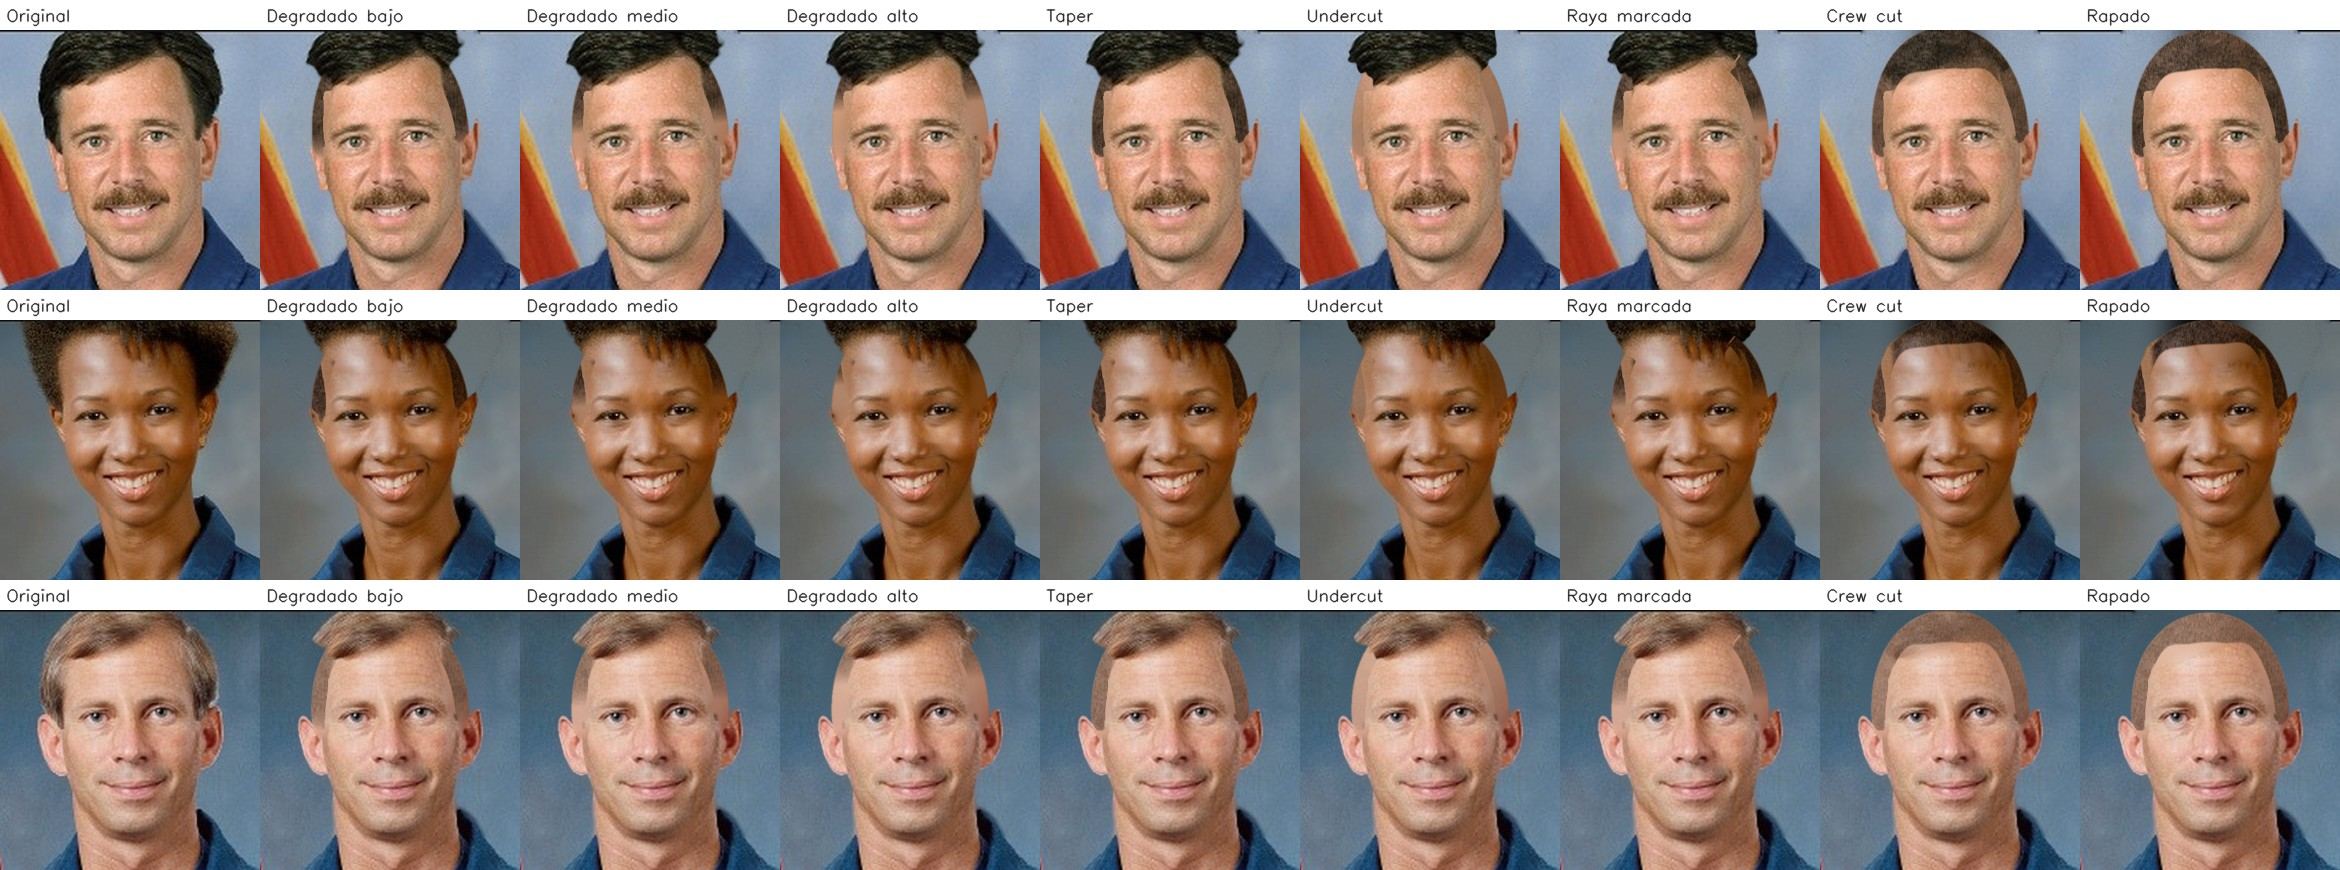
\includegraphics[width=\linewidth]{cortes.jpg}
  \caption{Los ocho cortes sobre tres retratos de dominio público.}
  \label{fig:cortes}
\end{figure}

\subsection{Tinte y segmentación del pelo}

La figura~\ref{fig:tinte} compara las máscaras del YOLO propio y de MediaPipe, y el tinte con cada una:
\begin{itemize}
  \item las dos máscaras coinciden en la mayor parte del pelo;
  \item el YOLO propio tiende a incluir más borde y más mechones finos.
\end{itemize}
Medida como IoU entre las máscaras sin refinar, la coincidencia fue de 0{,}82 a 0{,}94 en siete retratos de prueba. Dentro de la aplicación, que compara la máscara refinada de YOLO con la de MediaPipe, el valor reportado varió entre 0{,}58 (pelo muy corto y rizado) y 0{,}96. El tinte conserva la textura del pelo y logra tanto aclarar como oscurecer.

\begin{figure}[ht]
  \centering
  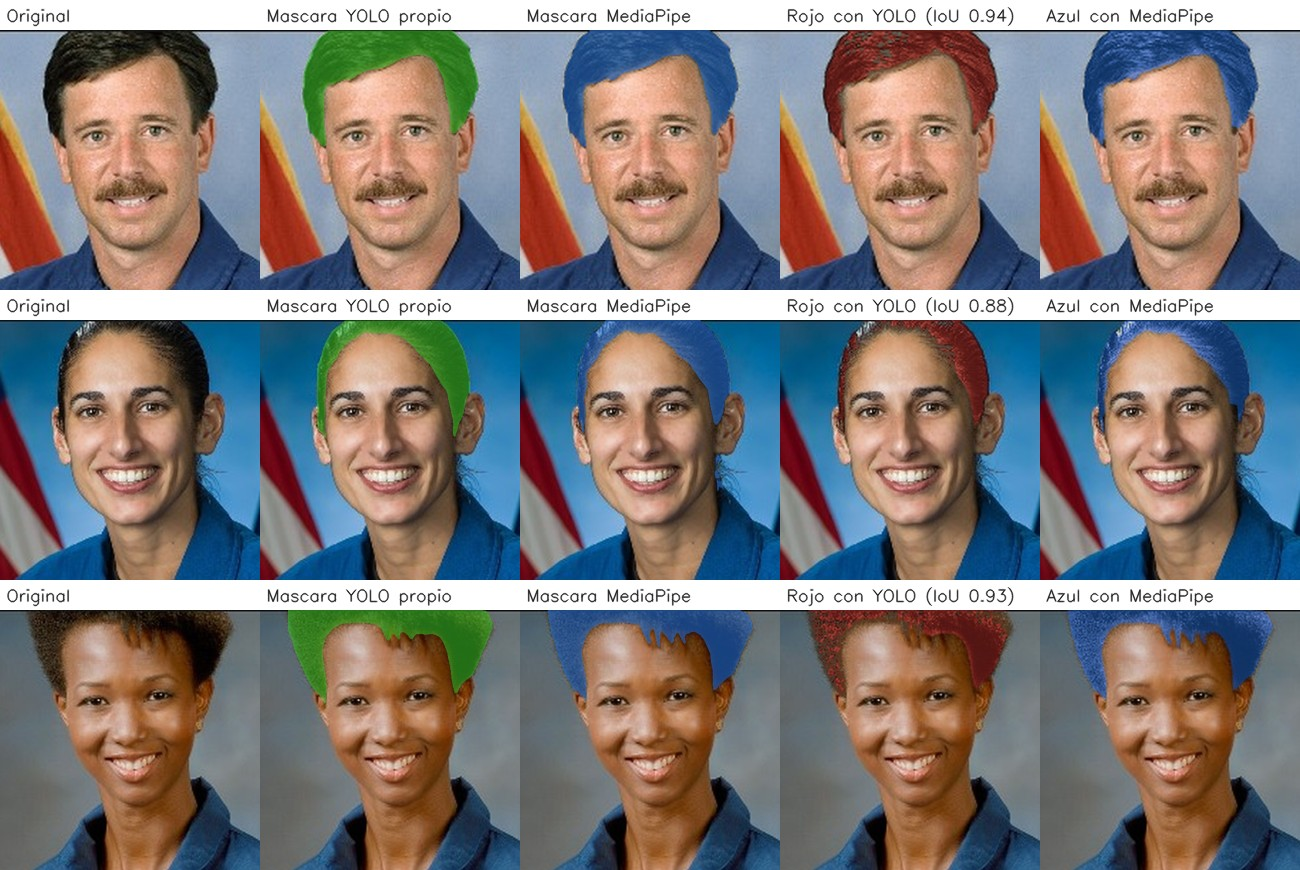
\includegraphics[width=0.95\linewidth]{tinte_modelos.jpg}
  \caption{Máscara del YOLO propio (verde) y de MediaPipe (azul), y el tinte con cada una. El título de la cuarta columna indica la IoU entre ambas máscaras.}
  \label{fig:tinte}
\end{figure}

\subsection{Tinte de la barba}

La figura~\ref{fig:barbatinte} muestra el tinte de barba en dos casos: una barba puesta por la propia aplicación, que se tiñe entera usando la máscara de su estilo, y un bigote real, detectado por textura.

\begin{figure}[ht]
  \centering
  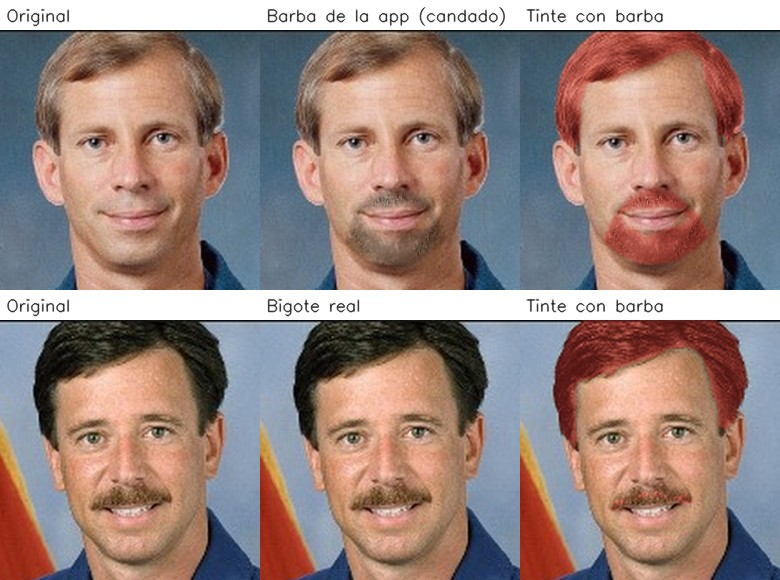
\includegraphics[width=0.62\linewidth]{barba_tinte.jpg}
  \caption{Tinte de barba. Arriba, un candado puesto por la aplicación; abajo, un bigote real.}
  \label{fig:barbatinte}
\end{figure}

\subsection{Gaussianas 2D}

La tabla~\ref{tab:psnr} resume la calidad de la reconstrucción en seis retratos. La relación señal/ruido de pico (PSNR) crece casi linealmente con $\log N$: unos 8~dB por cada multiplicación por diez del número de gaussianas (figura~\ref{fig:psnr}).

\begin{table}[ht]
\centering
\small
\begin{tabular}{@{}rccc@{}}
\toprule
Gaussianas & PSNR medio (dB) & Rango (dB) & Tiempo medio (s) \\
\midrule
20 & 18{,}4 & 16{,}7 -- 20{,}2 & 0{,}9 \\
60 & 22{,}2 & 20{,}3 -- 24{,}9 & 2{,}4 \\
200 & 26{,}0 & 24{,}1 -- 28{,}4 & 4{,}1 \\
600 & 29{,}8 & 27{,}5 -- 31{,}8 & 3{,}8 \\
2000 & 34{,}5 & 32{,}9 -- 35{,}9 & 3{,}6 \\
\bottomrule
\end{tabular}
\caption{Reconstrucción de retratos con gaussianas 2D.}
\label{tab:psnr}
\end{table}

\begin{figure}[ht]
  \centering
  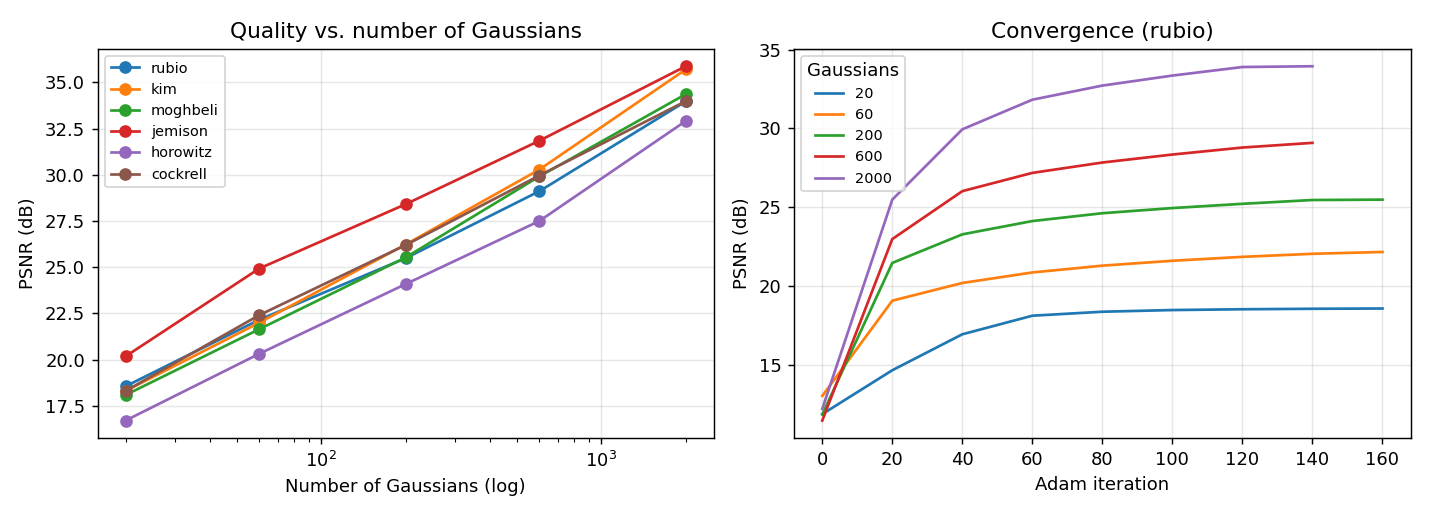
\includegraphics[width=0.85\linewidth]{psnr.png}
  \caption{PSNR en función del número de gaussianas y convergencia por iteración.}
  \label{fig:psnr}
\end{figure}

\subsection{Contrarreloj}

Para validar el juego se programó un ``bot barbero'' que recorre en zigzag la zona que hay que afeitar y levanta la máquina en los saltos largos (tabla~\ref{tab:juego}). Un bot que corta sin levantar la máquina, cruzando el objetivo, obtiene 0~puntos. Esto confirma que el puntaje premia afeitar con cuidado.

\begin{table}[ht]
\centering
\small
\begin{tabular}{@{}lccc@{}}
\toprule
Retrato y objetivo & Puntaje & Limpieza & Conservación \\
\midrule
rubio, candado & 827 & 0{,}83 & 0{,}99 \\
rubio, bigote & 814 & 1{,}00 & 0{,}81 \\
rubio, collar & 690 & 0{,}69 & 1{,}00 \\
kim, candado & 817 & 0{,}83 & 0{,}99 \\
horowitz, collar & 656 & 0{,}66 & 1{,}00 \\
cockrell, bigote & 646 & 0{,}98 & 0{,}66 \\
\bottomrule
\end{tabular}
\caption{Resultados del bot barbero.}
\label{tab:juego}
\end{table}

\subsection{Interfaz}

La interfaz (figuras~\ref{fig:inicio}, \ref{fig:ui} y~\ref{fig:ficha}) organiza las herramientas en cuatro grupos: \emph{Estilos}, \emph{3D}, \emph{Juegos} y \emph{Mis looks}. La foto es compartida entre todas las herramientas y cada resultado se ve en un comparador antes/después. La tarjeta ``Tu cara'' muestra la forma detectada y marca los estilos sugeridos. La interfaz se adapta al celular.

\begin{figure}[ht]
  \centering
  \begin{subfigure}{0.49\linewidth}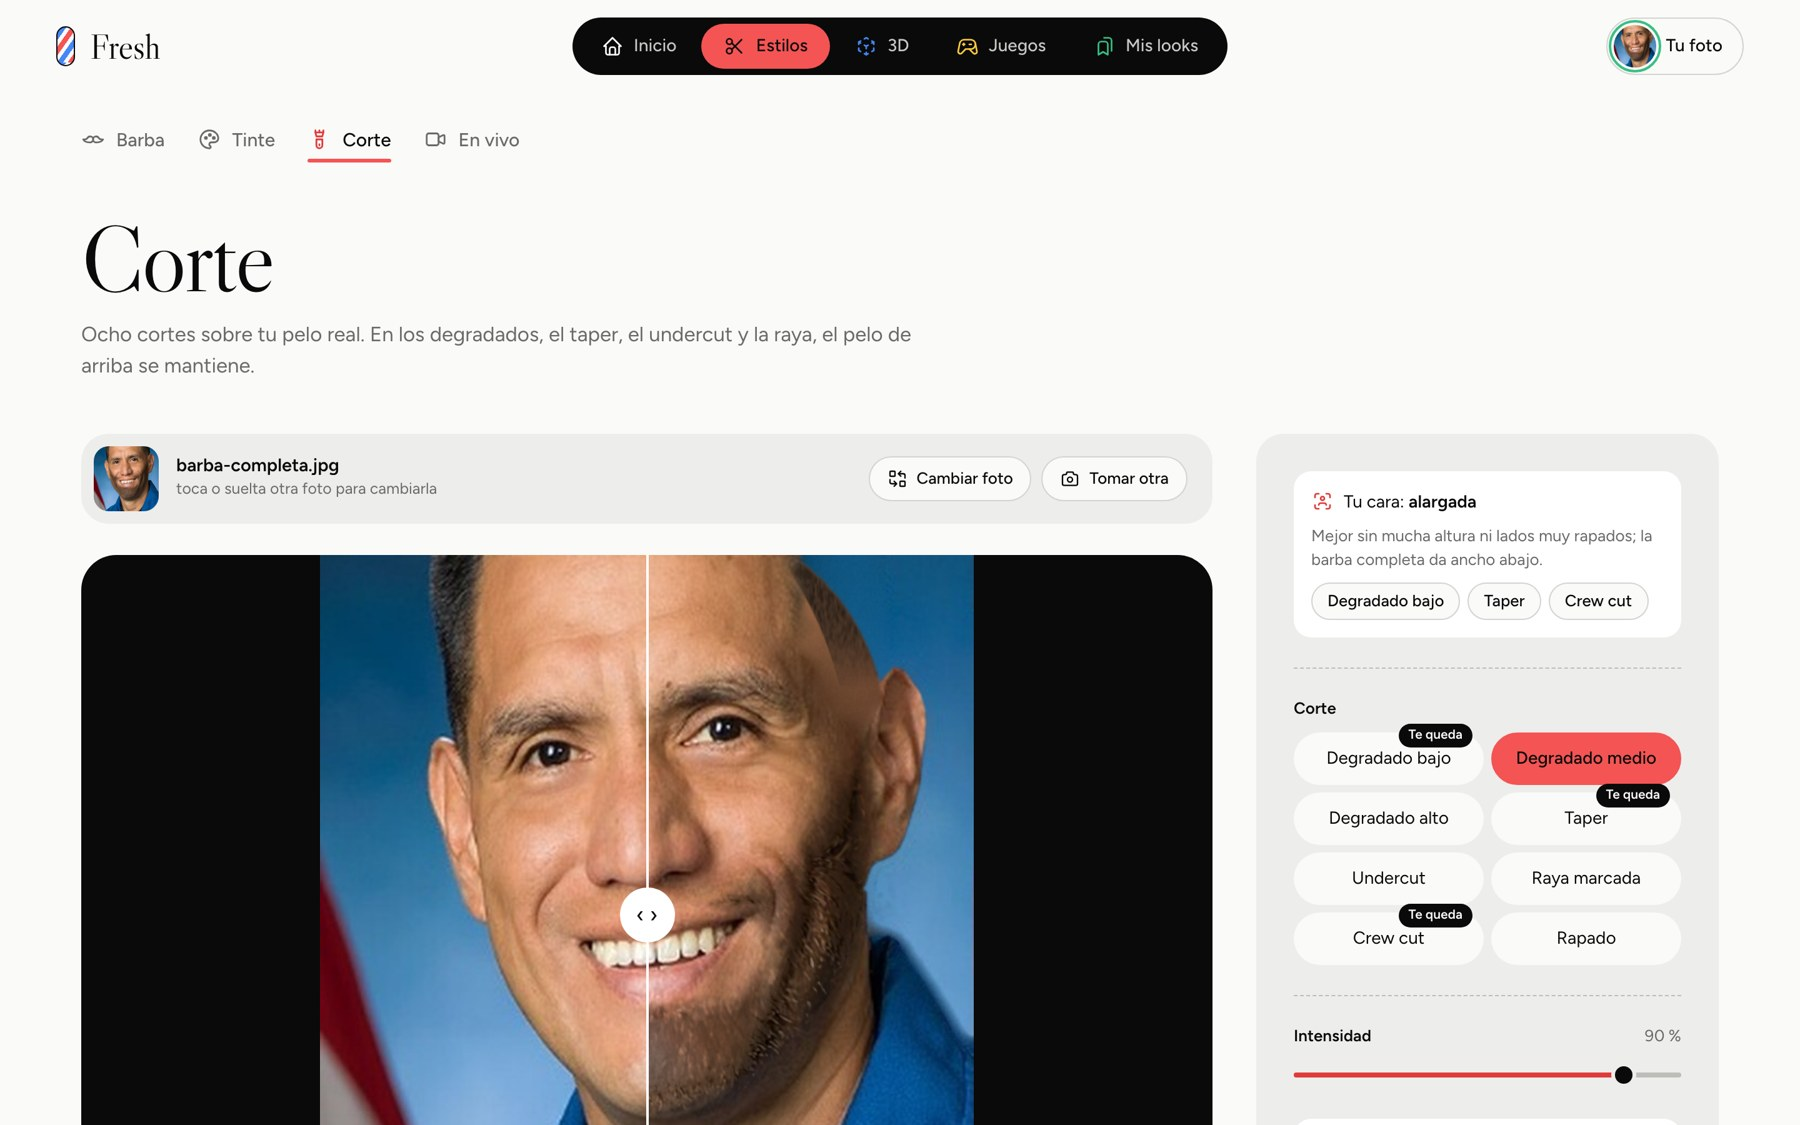
\includegraphics[width=\linewidth]{ui_corte.jpg}\caption{Corte, con sugerencias por forma de cara}\end{subfigure}\hfill
  \begin{subfigure}{0.49\linewidth}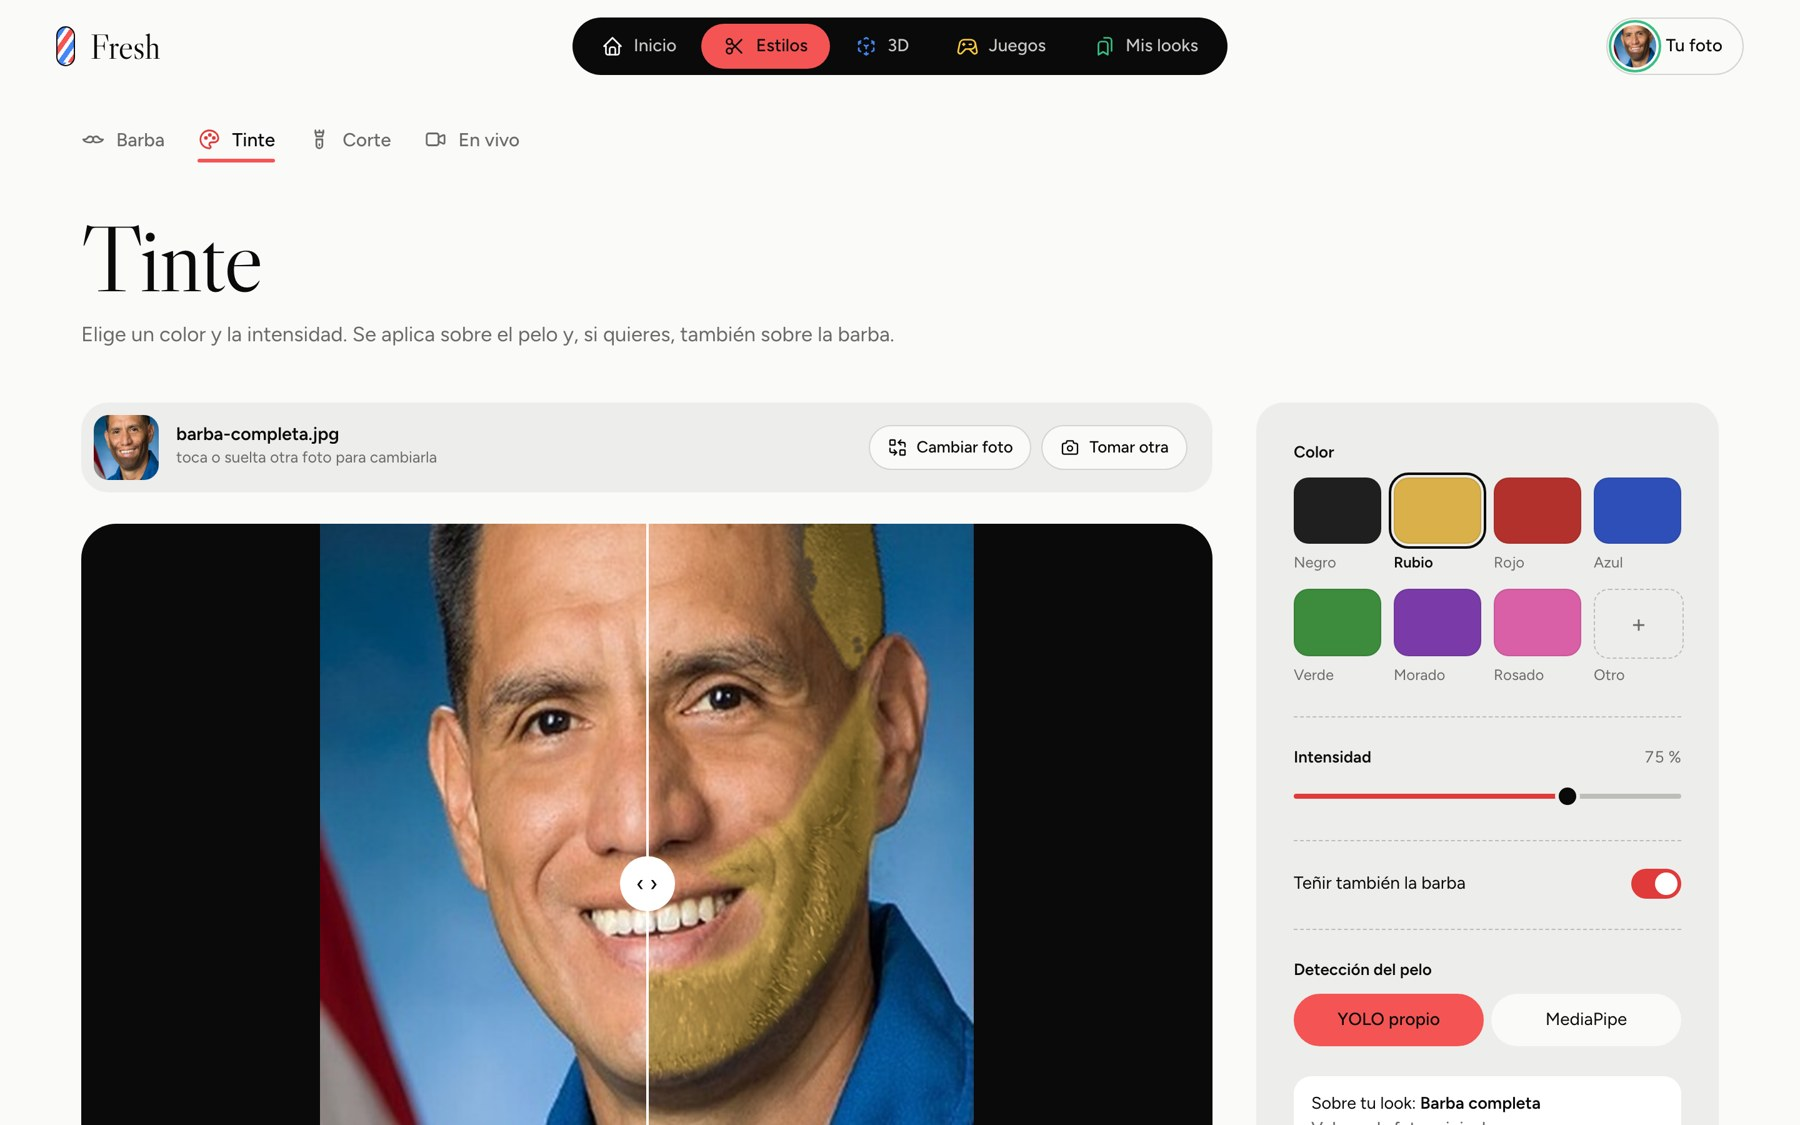
\includegraphics[width=\linewidth]{ui_tinte.jpg}\caption{Tinte con barba y selector de modelo}\end{subfigure}
  \caption{Paneles de Corte y Tinte sobre un look combinado.}
  \label{fig:ui}
\end{figure}

\begin{figure}[ht]
  \centering
  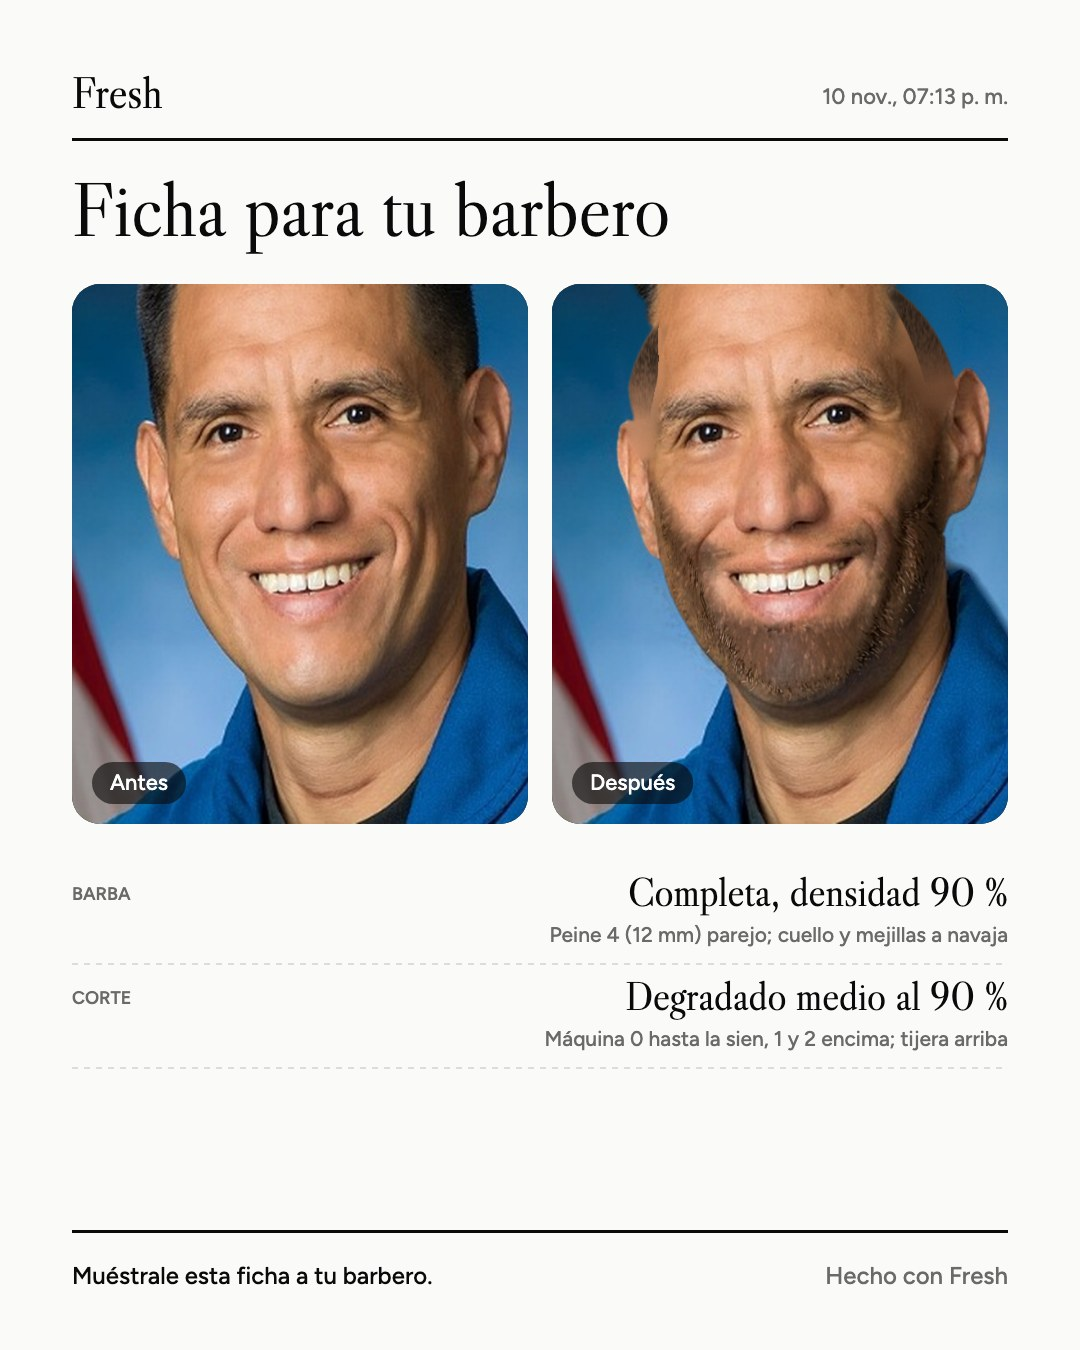
\includegraphics[width=0.45\linewidth]{ui_ficha.jpg}
  \caption{Ficha para el barbero de un look combinado, con indicaciones de máquina por servicio.}
  \label{fig:ficha}
\end{figure}

\subsection{Rendimiento}

La tabla~\ref{tab:tiempos} reúne los tiempos medidos. Las fotos más grandes que 2048~px se reducen al recibirlas: una foto de 4000~px tardaba 18~s en el contenedor y ahora tarda menos de 1~s.

\begin{table}[ht]
\centering
\small
\begin{tabularx}{\linewidth}{@{}X r@{}}
\toprule
Operación & Tiempo \\
\midrule
Corte, fotos de 1024 a 1638~px (contenedor Docker, CPU) & 0{,}6 -- 1{,}9~s \\
Corte, foto de 4000~px (contenedor Docker) & 0{,}8 -- 1{,}1~s \\
Corte, foto de 600~px (Apple M5, local) & 0{,}1 -- 0{,}3~s \\
Tinte con YOLO y barba (contenedor Docker, modelo ya cargado) & 2{,}5~s \\
Construcción del espejo 3D (unas 105\,000 gaussianas) & 2{,}6~s \\
Barba en vivo, por cuadro & 61~ms \\
Física de la barba en vivo, por cuadro & 72~ms \\
\bottomrule
\end{tabularx}
\caption{Tiempos medidos.}
\label{tab:tiempos}
\end{table}

\subsection{Pruebas automáticas}
\label{sec:pruebas}

El proyecto tiene 53 pruebas con pytest, que GitHub Actions ejecuta en cada cambio:
\begin{itemize}
  \item 32 de la API y de los módulos de estilo;
  \item 10 de \emph{splatting} y física;
  \item 5 de la transferencia de pelo;
  \item 4 de la triangulación de Delaunay;
  \item 2 del laboratorio.
\end{itemize}

Entre otras cosas, verifican:
\begin{itemize}
  \item \textbf{Delaunay}: ningún punto cae dentro de un círculo circunscrito, hay $2n-2-h$ triángulos, una grilla da exactamente los triángulos esperados sin superposiciones, los puntos colineales no generan triángulos y Fortune contiene todos los triángulos de Bowyer--Watson;
  \item \textbf{cortes}: ningún corte toca la cara; con intensidad 0 la foto no cambia; los píxeles lejos del pelo no cambian; un estilo desconocido da error;
  \item \textbf{entradas inválidas}: sin cara, la API responde 422, y con un estilo o modelo desconocido, 400;
  \item \textbf{forma de la cara}: la clasificación es correcta en proporciones sintéticas y todas las sugerencias corresponden a estilos existentes;
  \item \textbf{tinte de barba}: no tiñe piel limpia;
  \item \textbf{gaussianas 2D}: más gaussianas dan mayor PSNR;
  \item \textbf{física}: se asienta en reposo y se atrasa al mover la raíz;
  \item \textbf{espejo 3D}: las covarianzas son semidefinidas positivas y el \texttt{.ply} reconstruye exactamente la covarianza original;
  \item \textbf{juego}: no corta nada con la máquina apagada y conserva su objetivo entre cuadros;
  \item \textbf{servidor}: corre un solo proceso, para no partir el estado del modo en vivo y del juego.
\end{itemize}
Además, la aplicación arranca y aprueba las pruebas tanto con YOLO instalado como sin él.

\section{Limitaciones y trabajo futuro}
\label{sec:limitaciones}

\textbf{Limitaciones conocidas.}
\begin{itemize}
  \item \textbf{Oclusiones.} Si una mano pasa delante de la cara en el modo en vivo, la barba se dibuja encima de la mano.
  \item \textbf{Pelo sobre los ojos.} En el rapado y el \emph{crew cut}, si un flequillo largo tapa un ojo, quedan mechones sueltos, porque no se borra pelo dentro del polígono de la cara para no inventar el ojo.
  \item \textbf{Orejas tapadas.} Si el pelo tapaba las orejas, el rapado pone pelo corto donde irían las orejas, porque no hay información para reconstruirlas.
  \item \textbf{Barbas muy densas.} En barbas reales muy negras y tupidas, el tinte a veces toma solo los bordes: la textura no se distingue dentro de una zona uniforme.
  \item \textbf{Una sola vista en el espejo 3D.} El espejo se construye desde una foto: no tiene nuca, y con giros de más de unos 40° se estira el relieve detrás de la cara.
  \item \textbf{Velocidad en vivo.} El modo en vivo corre a unos 10 cuadros por segundo; con giros rápidos la barba se atrasa un poco.
  \item \textbf{Clasificación de la cara.} Es una heurística calibrada estadísticamente, no un diagnóstico; caras en el límite entre dos formas pueden caer en cualquiera de ellas.
  \item \textbf{Un solo usuario en vivo.} El estado del modo en vivo es único por servidor: dos cámaras a la vez compartirían el anclaje.
\end{itemize}

\textbf{Trabajo futuro.}
\begin{itemize}
  \item Tinte en vivo en el navegador con un \emph{shader} de WebGL y segmentación en JavaScript, para llegar a 30 cuadros por segundo sin servidor.
  \item Optimizar las gaussianas 3D con varias vistas (3DGS entrenado) para completar la cabeza.
  \item Segmentar la barba con un modelo propio, entrenado con las máscaras de CelebAMask-HQ.
  \item Estado del modo en vivo por sesión, para varios usuarios a la vez.
\end{itemize}

\section{Conclusiones}
\label{sec:conclusiones}

Fresh muestra que un probador de barbería creíble se puede construir con técnicas clásicas de computación gráfica, sin modelos generativos y sin GPU. La clave fue modelar la geometría de la persona en lugar de pegar imágenes:
\begin{itemize}
  \item una malla de Delaunay propia permite deformar barbas reales sobre cualquier cara;
  \item separar luminosidad y color en CIELAB permite teñir sin perder los mechones;
  \item un marco de la cabeza medido en anchos de cabeza, junto con un relleno \emph{pull-push} que elige sus fuentes, permite quitar y volver a crear el pelo para ocho cortes distintos.
\end{itemize}

Las gaussianas resultaron ser una representación versátil a lo largo del proyecto: dibujan pelos sueltos en la barba con física, reconstruyen un retrato en 2D, forman una cabeza 3D girable y una peluca multivista, y siempre con el mismo principio de proyectar, acumular y componer.

Varias decisiones se tomaron midiendo:
\begin{itemize}
  \item el anclaje de la textura a la malla redujo el deslizamiento de la barba en vivo, medido con flujo óptico \cite{farneback2003}, de 2{,}88 a 1{,}11;
  \item el cambio de Telea a \emph{pull-push} eliminó el pelo fantasma;
  \item calibrar la forma de la cara con 419 caras evitó que todas cayeran en la misma clase;
  \item limitar el tamaño de entrada bajó de 18~s a menos de 1~s el tiempo de una foto de celular.
\end{itemize}

El producto está terminado y se puede reproducir:
\begin{itemize}
  \item tiene interfaz para escritorio y celular;
  \item tiene 47 pruebas automáticas e integración continua;
  \item se levanta con un solo comando de Docker;
  \item incluye el modelo de segmentación entrenado por el equipo.
\end{itemize}
Las limitaciones que quedan (oclusiones, una sola vista en 3D, pelo que tapa los ojos o las orejas) marcan el camino para seguir mejorándolo.


\bibliographystyle{ieeetr}
\bibliography{references}

\appendix
\section{API del servidor}
\label{sec:anexo-api}

Todos los \emph{endpoints} reciben \texttt{multipart/form-data} y viven bajo \texttt{/api}.

\begin{table}[ht]
\centering
\small
\begin{tabularx}{\linewidth}{@{}l X@{}}
\toprule
\emph{Endpoint} & Uso \\
\midrule
\texttt{GET /health} & Estado del servidor y si el YOLO propio está disponible. \\
\texttt{POST /face-shape} & Forma de la cara, proporciones y estilos sugeridos (JSON). \\
\texttt{POST /beard} & Barba sobre una foto (\texttt{style}, \texttt{strength}). \\
\texttt{POST /dye} & Tinte (\texttt{color}, \texttt{strength}, \texttt{beard}, \texttt{beard\_style}, \texttt{model}). Devuelve en cabeceras el modelo usado y la IoU con MediaPipe. \\
\texttt{POST /haircut} & Corte (\texttt{style}, \texttt{strength}). \\
\texttt{POST /mesh} & Malla de Delaunay dibujada sobre la foto. \\
\texttt{POST /live} & Un cuadro del modo en vivo (tinte, barba, malla o física). \\
\texttt{POST /gaussians} & Retrato con $N$ gaussianas 2D. \\
\texttt{POST /game/start}, \texttt{/game/frame} & Ronda de Contrarreloj. \\
\texttt{POST /head3d} & Gaussianas 3D del espejo, o archivo \texttt{.ply}. \\
\texttt{POST /transfer/*} & Escaneo, reconstrucción, cara 3D, fotos y peluca de gaussianas. \\
\texttt{POST /lab/build}, \texttt{/lab/mesh} & Avatar del laboratorio. \\
\texttt{GET /models/face\_landmarker.task} & Modelo de malla facial para el navegador. \\
\bottomrule
\end{tabularx}
\caption{\emph{Endpoints} principales.}
\end{table}

\section{Estructura del código}

\begin{lstlisting}
backend/
  app/
    api/routes.py          endpoints
    core/pipeline.py       orquestacion
    core/detection/        cara, puntos, mano, filtro One-Euro
    core/segmentation/     pelo (MediaPipe, YOLO), barba, mascaras
    core/geometry/         Delaunay (Fortune, Bowyer-Watson), warp, forma de cara
    core/coloring/         tinte en CIELAB
    core/compositing/      barba, fisica, corte, cabeza sin pelo
    core/splatting/        gaussianas 2D, cabeza 3D, peluca 3D, cara 3D
    core/game/             Contrarreloj
    core/lab/              avatar en vivo
  models/                  modelos de MediaPipe y hair_best.pt
  tests/                   49 pruebas con pytest
  training/                preparacion de datos y entrenamiento de YOLO
frontend/
  index.html, css/, js/    interfaz y visor WebGL2
docs/                      documentacion tecnica y capturas
report/                    este documento en LaTeX
Dockerfile, docker-compose.yml, run.sh
\end{lstlisting}


\end{document}
